\pdfminorversion=7
\documentclass[final,5p,times,number]{elsarticle}

\usepackage{amsmath,amssymb,amsfonts}
\usepackage[ruled,vlined,linesnumbered]{algorithm2e}
\usepackage{textcomp}
\usepackage{xcolor}
\usepackage{booktabs}
\usepackage{listings}
\usepackage{url}
\usepackage{multirow}
\usepackage{tabularx}
\usepackage{lmodern}
\usepackage[final]{microtype}
\usepackage{tikz}
\usetikzlibrary{arrows.meta,positioning,fit,calc}
\graphicspath{{./}}
\emergencystretch=2em

\biboptions{sort&compress}

\journal{Computers \& Security}

\begin{document}

\begin{frontmatter}

\title{LoopFuzz: Closed-Loop Runtime Admission Control for LLM-Guided Stateful Protocol Fuzzing}

\author[inst1]{Ketang Chen}
\ead{3250006913@student.must.edu.mo}
\author[inst1]{Xiaolei Ren\corref{cor1}}
\ead{xlren@must.edu.mo}
\cortext[cor1]{Corresponding author: Xiaolei Ren. Email address: xlren@must.edu.mo}

\affiliation[inst1]{organization={Macau University of Science and Technology},
            addressline={Avenida Wai Long, Taipa},
            city={Macau},
            country={China}}

\begin{abstract}
Stateful protocol fuzzing is difficult because a syntactically valid message can still violate the current session state, especially when a large language model (LLM) can inject candidates into a long-running campaign. We present LoopFuzz, a closed-loop runtime admission-control design for LLM-guided stateful protocol fuzzing. LoopFuzz treats model outputs as bounded hypotheses rather than queue entries. It admits an intervention only when runtime evidence supports parseability, response-grounded acceptability, state reachability, and downstream gain. Failed executions become counterexamples for local refinement, and state-aware scheduling triggers model assistance only under adaptive plateau conditions. Re-audited run summaries answer a scoped lineage question: within the AFLNet/ChatAFL implementation and measurement lineage, the integrated LoopFuzz control strategy improves state exploration and improves absolute branch coverage on most primary targets. Auxiliary NSFuzz artifacts and a Mosquitto-only MBFuzzer worker archive are retained as external diagnostics rather than homogeneous rankings. The archive does not include same-format StateAFL, Bleem, Logos, or MBFuzzer rows for the primary table, nor a full no-admission ablation. The evidence therefore supports a bounded claim about the evaluated integrated strategy, not an isolated proof of the admission formula or an overall advantage over specialized state-aware fuzzers.
\end{abstract}

\begin{keyword}
Protocol fuzzing \sep Large language models \sep Runtime admission control \sep Stateful testing \sep Counterexample-guided refinement
\end{keyword}

\end{frontmatter}

\section{Introduction}
Network protocol implementations remain difficult security targets because correctness depends on interaction history rather than isolated inputs~\cite{aflnet,stateafl,sgf_usenix22,formatted_stateful_greybox_fuzzing_2024,resolverfuzz_query_response_2024}. An FTP server, for example, rejects a well-formed \texttt{PASS} command if no valid \texttt{USER} command has established the login state. Unlike file fuzzing, protocol fuzzing must preserve message syntax, temporal order, and request-response progress across a multi-step session~\cite{resolverfuzz_query_response_2024,mbfuzzer_mqtt_2025,bleem_packet_sequence_2023,logos_log_guided_fuzzing_2024,diane_identifying_fuzzing_triggers_2021,corecrisis_context_aware_2025}.

Traditional coverage-guided fuzzers work well for stateless parsers. They fit network servers poorly when later behavior depends on earlier valid exchanges~\cite{directed_greybox_fuzzing_2017,seed_selection_successful_fuzzing_2021,one_fuzzing_strategy_rule_2022,regression_greybox_fuzzing_2021,efficient_errors_2022}. Stateful greybox fuzzers such as AFLNet and StateAFL partially close this gap. They infer progress from responses and replay valid traces~\cite{aflnet,stateafl,sgf_usenix22,profuzzbench_benchmark_stateful_protocol_2021,snapfuzz_high_throughput_fuzzing_2022,bleem_packet_sequence_2023,formatted_stateful_greybox_fuzzing_2024}. Even so, byte-level mutation still struggles to synthesize the context-sensitive messages needed to cross deep protocol boundaries.

Large language models offer a plausible source of such messages. ChatAFL and later LLM-assisted fuzzers show that a model can extract structure from specifications, logs, or documentation and produce fluent candidates~\cite{chatafl,fuzz4all_universal_fuzzing_large_2024,llmif_augmented_large_language_2024,matter_llm_specification_2024,carpetfuzz_documentation_2023,prompt_fuzzing_fuzz_driver_2024,large_language_models_are_2023,large_language_models_are_2024}. But fluency is not enough. A request can be grammatically plausible and still be invalid for the live session state. Such executions spend budget without improving queue quality.

LoopFuzz places a runtime admission controller between LLM generation and queue admission. It treats the LLM as a hypothesis generator rather than an oracle. It derives message hypotheses from available RFC fragments, seed traces, and observed responses. It stores failed executions as counterexamples and uses them for counterexample-guided refinement (CEGR) rather than unconstrained regeneration. It also uses inferred protocol state machine (IPSM) feedback to prioritize frontier states and rare transitions, and to trigger assistance only when ordinary mutation stalls. The name \emph{LoopFuzz} emphasizes closed-loop admission and refinement, avoiding any suggestion of formal verification of protocol semantics, model behavior, or server correctness.

The contributions of this paper are as follows:
\begin{itemize}
    \item \textbf{Hypothesis-Driven Modeling.} LoopFuzz derives message grammars and field constraints from RFC fragments, seed traces, and observed responses, and maintains them as explicit runtime hypotheses.
    \item \textbf{Runtime Admission Boundary.} LoopFuzz inserts a runtime admission controller between the LLM and the queue. It checks structure before execution and uses bounded trial evidence to evaluate response acceptability, state reachability, and downstream gain before durable queue promotion. The current archive evaluates this boundary as part of an integrated controller rather than through a full no-admission ablation.
    \item \textbf{Counterexample-Guided Refinement.} LoopFuzz preserves failed request-response traces as counterexamples and uses them to patch one field constraint or production at a time, which constrains model freedom and stabilizes refinement.
    \item \textbf{State-Aware Scheduling.} LoopFuzz leverages IPSM topology, state productivity, and adaptive plateau detection to prioritize underexplored frontier states and to request model assistance only when mutation alone stalls.
    \item \textbf{Scoped Empirical Study.} We evaluate LoopFuzz on a repeated-run benchmark archive. The primary study asks whether the integrated control strategy changes final \texttt{b\_abs} and response-derived IPSM \texttt{edges} within the AFLNet/ChatAFL lineage. Auxiliary NSFuzz artifacts, Mosquitto-only MBFuzzer artifacts, and policy ablations are reported as scope-setting evidence rather than as a claim of overall superiority over StateAFL, NSFuzz, Bleem, Logos, MBFuzzer, or other specialized state-aware fuzzers. Because the archive lacks a \emph{LoopFuzz-no-admission} condition, the ablation evidence does not isolate the complete contribution of the $P/U/R/G$ admission formula.
\end{itemize}

Accordingly, the paper evaluates LoopFuzz as a campaign-control policy, not as a standalone message generator. In stateful protocol fuzzing, generation matters only when it survives runtime evidence and improves downstream queue quality.

\section{Background and Motivation}

\begin{table*}[ht]
\centering
\caption{Among the listed systems, LoopFuzz combines LLM hypotheses with runtime admission and online refinement; representative prior fuzzers differ in input prior, state signal, and admission boundary.}
\label{tab:taxonomy}
\renewcommand{\arraystretch}{1.3}
\footnotesize
\setlength{\tabcolsep}{3pt}
\resizebox{\textwidth}{!}{%
\begin{tabular}{l l c c l}
\toprule
\textbf{System} & \textbf{Input prior} & \textbf{State signal} & \textbf{Admission rule} & \textbf{Online refinement} \\
\midrule
Coverage-guided mutation fuzzing~\cite{directed_greybox_fuzzing_2017,seed_selection_successful_fuzzing_2021}         & Byte mutation & None & None & No \\
AFLNet~\cite{aflnet}              & PCAP mutation  & Response & Novelty & No \\
StateAFL~\cite{stateafl}          & PCAP mutation  & Memory & Novelty & No \\
ChatAFL~\cite{chatafl}            & LLM requests & History text & Direct admission & No \\
\textbf{LoopFuzz (ours)}         & \textbf{LLM hypotheses} & \textbf{IPSM frontier + validation} & \textbf{Runtime admission} & \textbf{Yes} \\
\bottomrule
\end{tabular}}
\normalsize
\end{table*}

Table~\ref{tab:taxonomy} contrasts LoopFuzz with representative fuzzers. Prior LLM-assisted protocol fuzzers improve input fluency, but they leave admission largely open-loop. We study a narrower question: does an integrated control strategy centered on runtime validation make LLM proposals more useful in a long-running stateful campaign?

\subsection{Coverage-Guided Fuzzing vs. Network Targets}
A coverage-guided fuzzer operates through a repeated feedback cycle of seed selection, mutation, execution, coverage measurement, and novelty-based queue update~\cite{seed_selection_successful_fuzzing_2021,one_fuzzing_strategy_rule_2022,regression_greybox_fuzzing_2021,efficient_errors_2022}.
This loop is effective for file parsers, but network targets impose three constraints that matter here:
\begin{enumerate}
    \item \textbf{Temporal state dependence:} server behavior depends on the order and semantics of earlier messages, not only on the current payload~\cite{aflnet,stateafl,sgf_usenix22,formatted_stateful_greybox_fuzzing_2024}.
    \item \textbf{Strict message format:} protocols require delimiters, field layouts, and often checksum or length consistency, so many mutated messages die before they reach deeper logic~\cite{gramatron_effective_grammar_aware_2021,griffin_grammar_free_dbms_2022,formatted_stateful_greybox_fuzzing_2024}.
    \item \textbf{Execution instability:} sockets, forking daemons, and asynchronous response handling complicate both coverage collection and campaign throughput~\cite{snapfuzz_high_throughput_fuzzing_2022}.
\end{enumerate}

\subsection{Stateful Greybox Fuzzing (SGF)}
SGF addresses this gap by treating the target as an \emph{inferred protocol state machine} (IPSM). Formally, the IPSM can be viewed as a Mealy machine $M = (Q, I, O, \delta, \lambda, q_0)$, where:
\begin{itemize}
    \item $Q$ is the set of inferred protocol states;
    \item $I$ is the set of client messages;
    \item $O$ is the set of observed server responses;
    \item $\delta$ maps a state and input to a successor state;
    \item $\lambda$ maps a state and input to an observed response; and
    \item $q_0$ is the initial connection state.
\end{itemize}

AFLNet-style fuzzers infer $Q$ from observed responses and use that structure to bias later exploration toward rare or promising parts of the protocol. Here, the IPSM matters for one reason. It gives LoopFuzz a notion of progress that is richer than raw edge coverage alone.

\subsection{LLM Integration into Protocol Fuzzing}
Large language models make it easier to propose structure-aware protocol messages from RFC text, interaction history, or observed responses. That helps with syntax and message diversity, but it does not solve the harder control problem: a fluent request can still be wrong for the live session state.

\subsection{A Motivating Example: Semantic Drift}

\begin{figure}[t!]
\centering
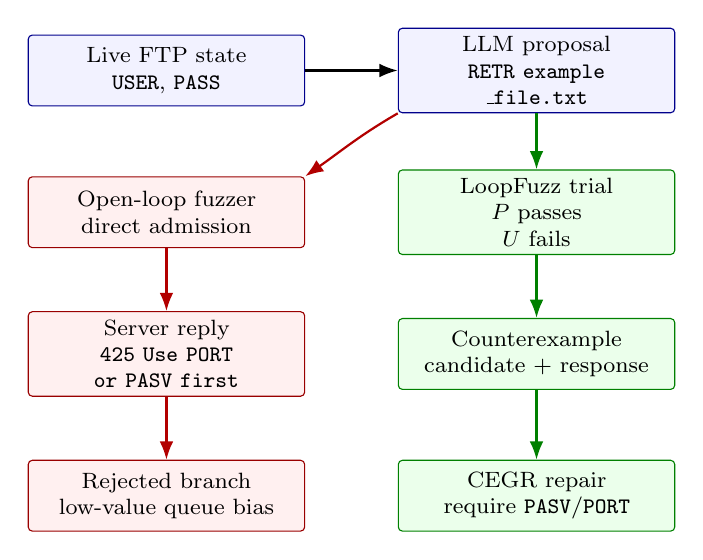
\begin{tikzpicture}[
    font=\footnotesize,
    >=Latex,
    box/.style={draw, rounded corners=1.5pt, align=center, minimum height=9mm, text width=33mm, fill=white, inner sep=3pt},
    open/.style={box, fill=red!6, draw=red!60!black},
    closed/.style={box, fill=green!8, draw=green!50!black},
    neutral/.style={box, fill=blue!5, draw=blue!55!black},
    arrow/.style={->, thick}
]
\node[neutral] (state) at (0,3.0) {Live FTP state\\\texttt{USER}, \texttt{PASS}};
\node[neutral] (llm) at (4.7,3.0) {LLM proposal\\\texttt{RETR example}\\\texttt{\_file.txt}};
\node[open] (openadmit) at (0,1.2) {Open-loop fuzzer\\direct admission};
\node[open] (reject) at (0,-0.6) {Server reply\\\texttt{425 Use PORT}\\\texttt{or PASV first}};
\node[open] (waste) at (0,-2.4) {Rejected branch\\low-value queue bias};
\node[closed] (gate) at (4.7,1.2) {LoopFuzz trial\\$P$ passes\\$U$ fails};
\node[closed] (cex) at (4.7,-0.6) {Counterexample\\candidate + response};
\node[closed] (repair) at (4.7,-2.4) {CEGR repair\\require \texttt{PASV}/\texttt{PORT}};
\draw[arrow] (state) -- (llm);
\draw[arrow, red!70!black] (llm.south west) to[out=210,in=35] (openadmit.north east);
\draw[arrow, red!70!black] (openadmit) -- (reject);
\draw[arrow, red!70!black] (reject) -- (waste);
\draw[arrow, green!50!black] (llm) -- (gate);
\draw[arrow, green!50!black] (gate) -- (cex);
\draw[arrow, green!50!black] (cex) -- (repair);
\end{tikzpicture}
\caption{Semantic drift in an FTP session. The model proposes \texttt{RETR} before the session opens a data channel. Open-loop fuzzing admits the rejected branch. LoopFuzz first checks local structure, then uses a bounded trial execution to observe the \texttt{425} response. The candidate is not promoted into the queue; the trace becomes a counterexample for repairing the missing \texttt{PASV}/\texttt{PORT} precondition.}
\label{fig:motivation}
\end{figure}

Consider an FTP fuzzing campaign against ProFTPD, as illustrated in Fig.~\ref{fig:motivation}. The fuzzer executes \texttt{USER} and \texttt{PASS}. It then queries the LLM for the next request. The model returns \texttt{RETR example\_file.txt}. The request is syntactically fluent but semantically premature. The client lacks an active data channel via \texttt{PASV} or \texttt{PORT}. The server rejects it with \texttt{425 Use PORT or PASV first}.

We call this failure \emph{semantic drift}. The request is locally plausible, but it violates the precondition of the current session state. An open-loop LLM fuzzer admits the request because it looks fluent. It then mutates a rejected branch instead of crossing the missing state transition. LoopFuzz handles this drift through runtime validation rather than through a purely pre-execution oracle. The controller first checks local structure and parseability, then performs a bounded trial execution whose \texttt{425} reply becomes negative evidence. The candidate is not promoted into the long-lived queue, and the failed trace is recorded as a counterexample. CEGR then repairs the missing \texttt{PASV}/\texttt{PORT} precondition instead of regenerating the full continuation. This example motivates the design claim: LLM assistance should be mediated by runtime evidence rather than by surface fluency alone. We use semantic drift as an operational motivation for selective queue admission and CEGR repair, not as a separately estimated global rate.

\section{Related Work}
We position LoopFuzz against the prior lines that are closest in mechanism and evaluation.

Earlier structure-aware fuzzing used explicit structure, inferred snippets, token constraints, or grammar guidance to preserve validity~\cite{snipuzz_black_box_fuzzing_2021,token_level_fuzzing_2021,gramatron_effective_grammar_aware_2021,griffin_grammar_free_dbms_2022,no_grammar_no_problem_2023,likely_invariants_feedback_2021,mundofuzz_grammar_inference_2022}. These systems improve input quality, but they do not address the control problem that arises when an external model proposes state-dependent protocol messages.

Stateful greybox and state-aware network-service fuzzing address protocol interaction more directly. AFLNet, StateAFL, NSFuzz, and the broader SGF line infer or expose state structure from server responses, process memory, or program variables~\cite{aflnet,stateafl,nsfuzz,sgf_usenix22,profuzzbench_benchmark_stateful_protocol_2021}. They then use that structure to prioritize rare or productive traces. These systems define the broader comparison landscape, but they do not all expose the same state abstraction, instrumentation path, or archived endpoint metrics.

Later systems extend this idea to packet-sequence exploration, format-sensitive protocol fuzzing, and communication-heavy environments~\cite{bleem_packet_sequence_2023,formatted_stateful_greybox_fuzzing_2024,logos_log_guided_fuzzing_2024,msgfuzzer_message_sequence_guided_2024,resolverfuzz_query_response_2024,mbfuzzer_mqtt_2025,fuzzusb_hybrid_stateful_fuzzing_2022,dtls_fuzzer_dtls_protocol_2022,edhoc_fuzzer_edhoc_protocol_2023,tron_fuzzing_linux_network_2025}. LoopFuzz asks a narrower question: given an AFLNet-style response-derived IPSM and the ChatAFL-style LLM proposal path, does an integrated runtime-admission strategy make the campaign more reliable? AFLNet and ChatAFL are therefore the closest implementation-lineage baselines. StateAFL, SGF, NSFuzz, Bleem, Logos, and MBFuzzer remain important external comparison points, but the archive lacks same-format reproductions for most of them, gives NSFuzz partly different artifact semantics, and contains MBFuzzer only as a Mosquitto worker archive without AFLNet-lineage \texttt{edges}. We treat that gap as a limitation and use the external rows to bound the claim.

Adjacent work studies state-aware or interaction-heavy fuzzing in robotic policies, firmware, Linux drivers, middleware, hardware, and embedded systems~\cite{pgfuzz_policy_guided_fuzzing_2021,android_smarttvs_vulnerability_discovery_2021,fuzzware_mmio_2022,statefuzz_linux_driver_2022,differential_fuzzing_data_distribution_2024,fuzzing_hardware_like_software_2022,coverage_guided_fuzzing_embedded_2023}. Although not all are protocol fuzzers, they reinforce the point that state feedback can dominate raw mutation quality.

Target-aware scheduling and semantic validation form another relevant line. Directed greybox fuzzing, seed selection, and strategy adaptation study how to steer budget toward high-value behaviors~\cite{directed_greybox_fuzzing_2017,windranger_blocks_2022,when_analysis_2025,seed_selection_successful_fuzzing_2021,one_fuzzing_strategy_rule_2022,regression_greybox_fuzzing_2021,efficient_errors_2022}. Semantic validation and fuzz-driver generation show that stronger inputs often require an explicit acceptance interface~\cite{one_engine_to_fuzz_em_all_2021,apicraft_fuzz_driver_2021}. LoopFuzz applies that lesson to LLM proposals.

Work on dependency inference, data-flow guidance, and learned signals outside protocol fuzzing also supports treating guidance as bounded evidence rather than as an oracle~\cite{rulf_rust_library_fuzzing_2021,smartian_analyses_2021,magneto_step_wise_approach_2024}.

LLM guidance addresses the synthesis bottleneck more directly. ChatAFL uses RFCs and interaction histories to generate protocol messages~\cite{chatafl}; adjacent systems use LLMs for general input generation, documentation-guided constraints, device fuzzing, or fuzz-driver generation~\cite{fuzz4all_universal_fuzzing_large_2024,llmif_augmented_large_language_2024,docter_documentation_guided_fuzzing_2022,carpetfuzz_documentation_2023,matter_llm_specification_2024,prompt_fuzzing_fuzz_driver_2024}. Our work is closest to ChatAFL, but adds a control boundary: LoopFuzz asks whether a proposal should be admitted, whether its hypothesis survives runtime evidence, and how the IPSM should guide the next query.

Benchmarking practice is also part of the context. ProFuzzBench established a reusable baseline for repeated protocol-fuzzing experiments~\cite{profuzzbench_benchmark_stateful_protocol_2021}. Recent methodology work shows how easily comparisons become unstable without fixed budgets, repeated trials, and careful interpretation of coverage signals~\cite{sok_prudent_evaluation_practices_2024,reliability_benchmarking_2022,many_stack_2022}. We follow that guidance because runtime-validated assistance is especially sensitive to campaign history.

\section{LoopFuzz Design}

Fig.~\ref{fig:arch} summarizes the three coupled loops in LoopFuzz: the Grammar Hypothesis Loop, the Fuzz Execution Loop, and the LLM Intervention Loop.

\begin{figure*}[t!]
\centering
\definecolor{lfblue}{RGB}{55,95,130}
\definecolor{lforange}{RGB}{178,108,35}
\definecolor{lfpurple}{RGB}{112,79,145}
\definecolor{lfgreen}{RGB}{67,128,93}
\definecolor{lfred}{RGB}{168,82,73}
\resizebox{\textwidth}{!}{%
\begin{tikzpicture}[
    font=\footnotesize,
    >=Latex,
    block/.style={draw, rounded corners=2pt, align=center, minimum height=9.2mm, text width=33mm, fill=white, inner xsep=3.5pt, inner ysep=3pt, line width=0.55pt},
    grammar/.style={block, draw=lfblue, fill=lfblue!7},
    fuzz/.style={block, draw=lforange, fill=lforange!8},
    llm/.style={block, draw=lfpurple, fill=lfpurple!7},
    gate/.style={block, draw=lfgreen, fill=lfgreen!9, text width=36mm, minimum height=10.5mm, line width=0.7pt},
    fail/.style={block, draw=lfred, fill=lfred!8},
    panel/.style={draw, rounded corners=4pt, line width=0.45pt},
    arrow/.style={->, line width=0.7pt, draw=black!68},
    feedback/.style={->, line width=0.7pt, dashed, draw=black!58},
    reject/.style={->, line width=0.7pt, draw=lfred!85!black},
    label/.style={font=\bfseries\footnotesize, align=center}
]
\draw[panel, draw=lfblue!45, fill=lfblue!3] (-5.80,-1.72) rectangle (-1.00,5.24);
\draw[panel, draw=lforange!50, fill=lforange!4] (-0.72,-1.72) rectangle (4.38,5.24);
\draw[panel, draw=lfpurple!45, fill=lfpurple!4] (4.88,-1.72) rectangle (9.48,5.24);

\node[label, text=lfblue] at (-3.40,4.86) {Grammar Hypothesis Loop};
\node[label, text=lforange] at (1.66,4.86) {Fuzz Execution Loop};
\node[label, text=lfpurple] at (7.24,4.86) {LLM Intervention Loop};
\draw[draw=lfblue!20, line width=0.45pt] (-5.44,4.42) -- (-1.36,4.42);
\draw[draw=lforange!22, line width=0.45pt] (-0.36,4.42) -- (4.02,4.42);
\draw[draw=lfpurple!20, line width=0.45pt] (5.24,4.42) -- (9.12,4.42);

\node[grammar] (evidence) at (-3.40,3.60) {RFC fragments\\seed traces\\observed responses};
\node[grammar] (hyp) at (-3.40,2.08) {Message hypotheses\\grammar and\\constraints};
\node[grammar] (tier1) at (-3.40,0.56) {Tier-1 sampling\\parsed-region check};
\node[fail] (cegr) at (-3.40,-0.96) {Tier-2 refinement\\counterexample patch};

\node[fuzz] (select) at (1.66,3.58) {State-aware\\seed selection\\frontier and productivity};
\node[fuzz] (exec) at (1.66,2.06) {Mutation and\\bounded execution};
\node[fuzz] (update) at (1.66,0.54) {Coverage and IPSM\\update};
\node[gate] (admit) at (1.66,-0.98) {Runtime admission\\pre-parse, trial\\evidence, queue};

\node[llm] (plateau) at (7.24,3.58) {Adaptive plateau\\budget check};
\node[llm] (prompt) at (7.24,2.06) {State prompt\\reuse filter and\\query isolation};
\node[llm] (reply) at (7.24,0.54) {Structured reply\\schema validation};
\node[llm] (dispatch) at (7.24,-0.98) {Bounded action\\mutation, priority, redirection};

\draw[arrow, draw=lfblue!85!black] (evidence) -- (hyp);
\draw[arrow, draw=lfblue!85!black] (hyp) -- (tier1);
\draw[reject] (tier1) -- node[right, font=\scriptsize, text=lfred!85!black] {counterexample} (cegr);
\draw[reject] (cegr.west) to[out=180,in=180,looseness=1.15] (hyp.west);

\draw[arrow, draw=lforange!85!black] (select) -- (exec);
\draw[arrow, draw=lforange!85!black] (exec) -- (update);
\draw[feedback, draw=lforange!85!black] (update.west) to[out=180,in=180,looseness=1.10] (select.west);

\draw[arrow, draw=lfpurple!85!black] (plateau) -- (prompt);
\draw[arrow, draw=lfpurple!85!black] (prompt) -- (reply);
\draw[arrow, draw=lfpurple!85!black] (reply) -- (dispatch);
\draw[feedback, draw=lfpurple!85!black] (update.east) to[out=20,in=200] node[above, font=\scriptsize, text=black!65] {growth rate} (plateau.west);

\draw[arrow, draw=lfgreen!80!black] (dispatch.west) -- (admit.east);
\draw[arrow, draw=lfgreen!80!black] (admit.north) -- (update.south);
\draw[feedback, draw=lfgreen!80!black] (admit.south) -- ++(0,-0.54) -| (select.south);
\draw[reject] (admit.west) -- node[above, font=\scriptsize, text=lfred!85!black, fill=white, inner sep=1pt] {reject} (cegr.east);
\end{tikzpicture}}
\caption{LoopFuzz changes the LLM from a queue producer into a bounded policy proposer. The Grammar Hypothesis Loop maintains message hypotheses, the Fuzz Execution Loop updates coverage and IPSM feedback, and the LLM Intervention Loop proposes bounded interventions. Runtime admission is two-stage: structural checks run before trial execution, while response, state, and coverage checks decide afterward whether the proposal can affect the queue.}
\label{fig:arch}
\end{figure*}

LoopFuzz preserves the stateful greybox fuzzing execution path. It sets a strict control boundary between LLM generation and durable queue admission. A model output changes the long-lived campaign only after runtime evidence supports admission. The admission rule has two stages: structural and local parseability checks run before a candidate is tried, and response behavior, inferred state reachability, and downstream campaign value are evaluated after a bounded trial execution. The method has four coupled components: grammar hypothesis generation, runtime admission control, counterexample-guided refinement, and state-aware scheduling.

This control boundary is the core idea of the paper. ChatAFL is open-loop: it uses a fixed trigger, a plain-text prompt, and direct admission of the extracted request. LoopFuzz is closed-loop: IPSM growth, state productivity, and hypothesis fitness determine when the LLM is queried, what context it receives, and whether a tried proposal is promoted into the campaign.

The three loops in Fig.~\ref{fig:arch} define the analytical roles of the method. The Grammar Hypothesis Loop constructs and repairs message hypotheses from RFC knowledge, seed traces, and observed responses. The Fuzz Execution Loop performs state selection, mutation, bounded execution, IPSM update, and novelty checking. The LLM Intervention Loop is activated only under plateau conditions and returns either a validated continuation or a bounded control action.

The remaining labels in Fig.~\ref{fig:arch} denote control interfaces rather than independent claims. Tier-1 sampling checks parsed execution regions, Tier-2 refinement repairs counterexamples, schema validation checks model replies, and bounded action dispatch maps an admitted action to mutation, seed-priority, or target-state control. The prompt reuse filter and query isolation bound repeated or failed model calls.

\subsection{Grammar Hypothesis Loop}
Let $\mathcal{L}(c, s, \Sigma)$ denote the LLM generation function under prompt context $c$, state summary $s$, and protocol knowledge $\Sigma$. LoopFuzz uses $\mathcal{L}$ in two stages. During initialization, it preserves ChatAFL's template extraction and seed enrichment path. Initial enrichment is scheduled as a bounded phase so that corpus diversification does not dominate early campaign time. During fuzzing, LoopFuzz adds a lazily initialized hypothesis layer. This layer is activated at the first plateau event and updated through sampled validation and refinement. The separation is important. The initialization phase broadens the initial seed set. Runtime hypotheses support runtime-validated control during long campaigns.

The Grammar Hypothesis Loop draws on three evidence sources when they are available: RFC fragments, queued seed traces or packet examples, and observed server responses, including response codes and error texts. For each message type $m$, the loop maintains a hypothesis $h_m=(G_m,\Phi_m)$. Here, $G_m$ is an ABNF-style or template-style production, and $\Phi_m$ is a set of field constraints. In LoopFuzz, $\Phi_m$ captures length bounds, enumerated values, token dependencies, and simple cross-field relations. This representation is more constrained than free-form text and lighter than a full formal protocol specification. We choose it because sampled online validation must remain cheap.

The evidence sources need not be complete. RFC fragments supply structure, seed traces provide executable examples, and observed responses provide target-specific evidence about rejection, progress, and state change. LoopFuzz therefore requires testable hypotheses, not a full formal protocol specification; runtime admission decides whether those hypotheses can affect the campaign.

\subsection{Runtime Admission Controller}
The runtime admission controller is the central mechanism in our design. It does not formally prove correctness, and it is not a purely pre-execution filter. Instead, it makes queue-admission decisions through two validation stages. Stage 1 checks whether a model proposal is structurally well formed and locally parseable before it is sent. Stage 2 performs a bounded trial execution and then evaluates the observed response, inferred state movement, and coverage or IPSM gain. A candidate intervention $x$ is retained only if
\[
A(x)=P(x) \land U(x) \land R(x) \land G(x),
\]
where $P$ denotes pre-trial local parseability, while $U$, $R$, and $G$ are post-trial predicates computed from the bounded execution: $U$ denotes response-grounded acceptability, $R$ denotes evidence of new or redirected state reachability, and $G$ denotes downstream gain in IPSM structure or coverage. If $P$ fails, the proposal is not executed. If $P$ passes but any post-trial predicate fails, the trial trace can be recorded as a counterexample or used to update state productivity, but the candidate is not promoted as a durable queue entry or accepted control action.

Table~\ref{tab:admission_predicates} gives the operational definition used to make this rule reproducible. The table separates the pre-trial structural gate from the post-trial evidence gates and lists the minimum event fields needed to replay an admission decision. These are the event-level fields that a complete artifact should preserve; as discussed in Section~\ref{sec:threats}, the current archive does not contain normalized admission-event logs from which cross-target admission-rate summaries can be reconstructed.

\begin{table*}[!t]
\centering
\caption{Operational definition of the $P/U/R/G$ admission predicates. $P$ is checked before a trial execution. $U$, $R$, and $G$ are computed from the bounded trial response, inferred state sequence, and coverage or IPSM novelty. A failed post-trial predicate can update counters, state productivity, or CEGR counterexamples, but it does not create a durable queue entry.}
\label{tab:admission_predicates}
{\scriptsize
\setlength{\tabcolsep}{3.0pt}
\renewcommand{\arraystretch}{1.12}
\resizebox{\textwidth}{!}{%
\begin{tabular}{>{\raggedright\arraybackslash}p{0.075\textwidth}
                >{\raggedright\arraybackslash}p{0.16\textwidth}
                >{\raggedright\arraybackslash}p{0.31\textwidth}
                >{\raggedright\arraybackslash}p{0.17\textwidth}
                >{\raggedright\arraybackslash}p{0.17\textwidth}
                >{\raggedright\arraybackslash}p{0.12\textwidth}}
\toprule
\textbf{Pred.} & \textbf{Input} & \textbf{Decision rule} & \textbf{Pass / fail example} & \textbf{Minimum audit fields} & \textbf{Execution and queue effect} \\
\midrule
\textbf{$P$}\\Parse. &
Schema-validated model reply; cleaned request or bounded action; current hypothesis $h_m=(G_m,\Phi_m)$; parsed message regions. &
Pass if the reply has a supported action type, required fields, valid field types and bounds, protocol delimiters or terminators, and a local parse under the current message hypothesis. Fail on malformed JSON/action objects, unknown action types, missing terminators, length/type violations, or local parser failure. &
Pass: \texttt{RETR file.txt} matches an FTP request template. Fail: missing command terminator, unknown action, or field length outside $\Phi_m$. &
event id; action and message type; schema flag; parse flag; parse error; hypothesis id. &
Exec.: no. Failure stops the candidate before execution. Success only makes it eligible for a bounded trial. \\
\midrule
\textbf{$U$}\\Accept. &
Trial response bytes, extracted response code or state id, timeout/disconnect status, and protocol adapter. &
Pass if the live response is not classified as a rejection sink. For text protocols whose states are three-digit response codes, 4xx/5xx are the default rejection class; target adapters or accumulated productivity evidence can override this when an apparent error state repeatedly yields paths. Timeouts, connection resets before a response, unparsable replies, and explicit \texttt{ERROR}/\texttt{BAD}/\texttt{invalid}/\texttt{denied} texts are negative evidence. &
Pass: FTP \texttt{230} login success or \texttt{227} passive-mode progress. Fail: FTP \texttt{425 Use PORT or PASV first}, timeout, or reset without response. &
response bytes; response code or state id; response class; timeout/disconnect; error hint; productivity; rejection reason. &
Exec.: yes, bounded. Failure blocks promotion and may lower hypothesis fitness or create a CEGR counterexample. \\
\midrule
\textbf{$R$}\\Reach. &
Trial state sequence extracted from responses, source state, scheduled target state or frontier state, and IPSM before the trial. &
Pass if the trial reaches a non-rejection protocol state, reaches the scheduled target state, moves out of a repeated rejection sink, or realizes a new response-derived state relation. Fail if it stays in the same rejection/error sink or produces no usable state sequence. This predicate answers whether the candidate reached a meaningful protocol state, regardless of whether it produced new code coverage. &
Pass: a candidate reaches the target passive-mode/data-channel state. Fail: repeated \texttt{425} leaves the execution in the same premature-transfer sink. &
source state; destination state; state sequence; target state; reached-target flag; new state relation; state productivity. &
Exec.: yes, bounded. Positive evidence updates IPSM/frontier statistics. Durable admission still requires $G$. \\
\midrule
\textbf{$G$}\\Gain &
Coverage bitmap result, branch/edge delta, IPSM path or edge novelty, queue-favored status, and the pre-trial campaign state. &
Pass if the trial yields measurable campaign novelty: a new coverage bitmap bit or branch, a new IPSM node/path/edge, or a seed that the fuzzer marks as favored because it improves the current corpus. Fail if the candidate is acceptable and reachable but only repeats an already saturated state with no coverage or IPSM novelty. &
Pass: \texttt{has\_new\_cov} or a new IPSM path is observed. Fail: an acceptable \texttt{NOOP} repeats a known state and exposes no new bitmap or IPSM signal. &
new bits; coverage flag; branch delta; new IPSM node/path/edge; favored flag; queue-promotion flag; gain reason. &
Exec.: yes, bounded. Only candidates passing $P$, $U$, $R$, and $G$ become durable queue entries or accepted controls. \\
\bottomrule
\end{tabular}}
}
\end{table*}

The distinction between $R$ and $G$ is intentional. $R$ asks whether the candidate can reach a meaningful protocol state under the response-derived IPSM. $G$ asks whether that execution produced measurable campaign novelty. A trial can therefore pass $U$ and $R$ yet fail $G$ when it reaches an already-known state without new coverage, IPSM, or queue value.

The cleanest ablation for this design would be \emph{LoopFuzz-no-admission}: it would keep the same model endpoint, prompts, query budget, plateau triggers, and scheduling policy, but skip the $P/U/R/G$ checks and directly enqueue or apply the model's suggested request or control action. Such a condition would isolate the contribution of the admission boundary from the rest of the control strategy. The current archive does not contain that condition. Therefore, our experiments evaluate LoopFuzz as an integrated control policy and do not independently prove the full causal effect of the admission formula.

The FTP example in Fig.~\ref{fig:motivation} illustrates the same two-stage logic. The candidate \texttt{RETR example\_file.txt} can satisfy local syntax under $P$, so LoopFuzz may try it in a bounded validation execution. The live \texttt{425} response then makes $U$ fail because no data channel has been negotiated. The trial also provides no useful new transition or coverage signal, so $R$ and $G$ do not support admission. LoopFuzz therefore declines to promote the candidate into the queue and records a counterexample that constrains CEGR to repair the missing \texttt{PASV}/\texttt{PORT} precondition.

\subsubsection{Structured Output and Parseability}
The plateau stage accepts either a concrete next-request candidate or a bounded structured-action object. Runtime validation first checks structural well-formedness, field types, length bounds, delimiter or terminator consistency, and action-schema consistency. LoopFuzz then tests local parseability against the current message hypotheses. It reuses parsed message regions already available during ordinary execution. This first stage can reject structurally invalid interventions before any trial execution. It does not decide whether a syntactically valid request is useful; that decision depends on the post-trial predicates in Table~\ref{tab:admission_predicates}.

\subsubsection{Response-Grounded Acceptability}
Parseability alone is insufficient. A parsed request can still be semantically premature. LoopFuzz therefore classifies the response observed during the bounded trial execution and treats a non-rejection response as positive evidence. For response-code protocols, 4xx/5xx states are the default rejection class; timeouts, early disconnects, unparsable replies, and explicit error texts are also negative evidence. The classification is conservative rather than absolute: a target adapter or accumulated productivity evidence can keep an apparent error state from becoming a permanent dead end if it repeatedly leads to new paths. Rejected or persistently unproductive responses reduce state productivity and hypothesis fitness. This gives an execution-grounded notion of acceptability rather than a semantic proof. The controller asks a narrow post-trial question: did live target behavior support promoting this candidate into the campaign?

\subsubsection{State Reachability and Coverage Gain}
The final admission question is whether the trial helped the campaign. LoopFuzz separates the answer into a state predicate and a novelty predicate. Reachability $R$ is computed from the response-derived state sequence: did the candidate reach a non-rejection state, the scheduled target state, or a new state relation? Gain $G$ is stricter and queue-facing: did that execution produce new coverage, a new IPSM node/path/edge, or a favored corpus entry? This separation handles the common case in which a candidate is state-valid but already saturated. The controller therefore uses IPSM-derived reachability and AFLNet-style novelty signals, not text quality alone. Fluent but repeatedly unproductive candidates may still consume a bounded validation execution, but they are filtered out before durable queue promotion instead of accumulating as low-value queue bias.

\subsection{Counterexample-Guided Refinement}
When sampled validation fails repeatedly, LoopFuzz records a concrete counterexample. The record contains the failure-triggering request fragment, the observed response, and the mismatch against the current hypothesis. Refinement is deliberately local. Instead of rewriting the full protocol description, the refinement interface constrains each repair to one field constraint or one production fragment. This single-patch discipline narrows the model's search space, limits unconstrained edits, and makes the repair path auditable. The resulting update is reintegrated into protocol matching and re-evaluated by later sampled validation.

This repair boundary is intentionally weaker than formal grammar repair. The one-field or one-production constraint is enforced through the refinement prompt and audit log, not through hard AST differencing. The current implementation also stores concrete failed traces without counterexample minimization. We therefore claim bounded local refinement, not complete protocol inference.

\subsection{State-Aware Scheduling and Plateau-Triggered Assistance}
Reducing malformed generations solves only half of the problem. Stateful fuzzers also stagnate when the campaign keeps revisiting locally dense IPSM regions while failing to cross narrow protocol bridges. LoopFuzz therefore treats IPSM feedback as a first-class scheduling signal.

To address this, LoopFuzz augments state selection with a frontier bonus $\beta$ derived from the out-degree of the IPSM:
\[
\beta = \begin{cases}
4.0 & \text{if } \deg^+(s) \le 1 \\
2.0 & \text{if } \deg^+(s) \le 3 \\
1.0 & \text{otherwise}
\end{cases}
\]
States absent from the IPSM receive the maximum bonus $\beta{=}4$. LoopFuzz then modulates this bonus with a three-level error-productivity hint: unknown, likely error, or confirmed productive. The reported implementation encodes these levels as 0, 1, and 2. This hint downweights frontier states that repeatedly behave like rejection sinks, but it does not discard them outright.

In the reported policy, hint level 1 applies a $\beta{\times}0.5$ penalty. Hint level 0 is reduced to $\beta{\times}0.7$ only after repeated low-productivity selections ($\mathit{selected\_times}{\ge}30$ and $\mathit{productivity}{<}0.005$). Hint level 2 receives no penalty. The hint is initialized from response-code classification and updated online. As a result, states can be promoted or demoted as evidence accumulates. They are not fixed by an early response pattern. This policy approximates a rare-transition preference without requiring an exact model of the full protocol state space.

These constants are the reported control policy, not a claim of global optimality. The frontier bonuses separate unseen or low-out-degree states from denser regions by coarse preference. The error-productivity penalties and the $(30,0.005)$ gate reduce repeated investment in response-derived rejection sinks while allowing recovery if later executions become productive. The $(80,30\%)$ node-stagnation safeguard and 64-call intervention budget prevent persistent hot-spot lock-in and unbounded LLM overhead. We report them for auditability, not as a full sensitivity analysis.

A complementary graph stagnation check tracks whether IPSM growth has collapsed at the graph level rather than only at the local state level. When no new nodes appear for an extended interval, the scheduler intermittently injects random selection to avoid persistent hot-spot lock-in. In the reported configuration, that safeguard activates after 80 consecutive rounds without node growth and uses a 30\% random-selection probability.

Plateau detection uses the IPSM edge growth rate $\dot{E}$, measured as edges gained per minute. LoopFuzz recalculates this rate every 60 seconds of wall-clock time and uses it to set an adaptive threshold:
\[
\tau(\dot{E}) = \begin{cases}
300 & \text{if } \dot{E} > 5 \\
200 & \text{if } 1 < \dot{E} \le 5 \\
150 & \text{if } \dot{E} \le 1
\end{cases}
\]
The initial value is $\tau{=}200$ for textual protocols. MQTT uses the higher thresholds $\{500,400,300\}$ under the same edge-growth bins because binary framing and broker-mediated behavior expose state progress more sparsely. More generally, LoopFuzz treats plateau triggering as a rate-sensitive control decision, not as a fixed-frequency query rule.

Assistance is invoked only when edge growth remains weak and the model-intervention budget is not exhausted. In the reported configuration, the plateau path opens when the unproductive streak reaches $\tau$ and prior model interventions remain below 64. Once inside that path, hypotheses are initialized lazily on first use. Refinement remains gated by validation count and accumulated counterexamples. The prompt reuse filter covers the most recent 64 LLM invocations. This prevents assistance from reacting to the same state summary again and again.

The plateau prompt exposes a compact state summary rather than a raw execution log. It includes IPSM node and edge counts, the current edge-growth rate, pending favored seeds, queued paths, the current target state, and the least productive states. The admissible action space is also bounded. A model can redirect the target state, reprioritize a small set of seeds, or propose bounded mutations over an existing seed. These actions are not admitted because they are fluent. They must still pass the same runtime admission boundary. This design keeps the LLM in the role of a state-directed policy proposer.

MQTT-specific scheduling is treated as a protocol adaptor, not as the general mechanism of LoopFuzz. For MQTT campaigns, packet-type selection uses a state-indexed action policy, and mutation-family selection uses a bandit-style controller. These signals help expose broker forwarding behavior to the IPSM, but they are protocol-adaptor details rather than primary performance-evaluation evidence. In short, assistance is conditional, budgeted, state-directed, and scoped by protocol evidence.

LoopFuzz also supports protocol-adaptor signals that are not headline evidence. For MQTT, the adaptor translates between binary packets and textual hypotheses, drives broker interactions, and records differential behavior across roles. A lightweight oracle can log authentication bypass, state-order violations, information leaks, traversal patterns, injection patterns, or denial-of-service indicators. These signals support auditing and triage, but they are not treated as confirmed vulnerabilities because crash deduplication, root-cause analysis, exploitability review, and oracle calibration are not normalized.

Algorithm~\ref{alg:fuzz} specifies the plateau path and the hypothesis-refinement gate. It formalizes how state-aware triggering, runtime admission checks, and CEGR interact within one campaign loop.

\begin{algorithm}[!tbp]
\caption{Runtime-Validated Plateau Recovery in LoopFuzz}
\label{alg:fuzz}
\SetAlgoLined
\SetAlgoNlRelativeSize{0}
\footnotesize
\DontPrintSemicolon
\KwIn{Target $T$, LLM interface $\mathcal{L}$, corpus $C$, edge-growth signal $\dot{E}$}
\KwOut{Coverage bitmap $\mathcal{B}_{global}$ and IPSM $\mathcal{M}$}
Initialize $\mathcal{B}_{global}$ and $\mathcal{M}$\;
\While{the campaign budget remains}{
    $s \leftarrow \textsc{SelectSeed}(C,\mathcal{M})$\;
    $(trace,Q) \leftarrow \textsc{MutateExecute}(T,s)$\;
    Update $\mathcal{B}_{global}$, $\mathcal{M}$, and frontier scores from $(trace,Q)$\;
    \If{sampled validation is due}{
        Validate active hypotheses on parsed regions of $Q$\;
    }
    \If{the adaptive plateau gate opens}{
        Initialize hypotheses on first use, if needed\;
        \If{counterexample evidence opens the refinement gate}{
            Patch the lowest-fitness hypothesis locally\;
        }
        $c \leftarrow \textsc{BuildPrompt}(\mathcal{M},C,Q,\dot{E})$\;
        \If{$c$ is not in the recent prompt cache}{
            $r \leftarrow \mathcal{L}(c)$ under process isolation\;
            Admit $r$ only if parseability, acceptability, reachability, and gain all hold\;
            Apply the admitted bounded action to $C$\;
        }
    }
}
\end{algorithm}

This integration imposes a bounded operating model. Initial enrichment is separated from long-running admission control, and hypothesis construction is deferred until the first plateau event. Model queries use process isolation, and network cleanup is bounded to limit persistent stalls on forking daemons. These mechanisms are operating conditions rather than separate novelty claims.

\section{Experimental Evaluation Design}

We organize the evaluation around three research questions that match the paper's main claims. The main experiment is a lineage experiment: it asks whether the integrated LoopFuzz control strategy changes a campaign that already has response-derived IPSM feedback and ChatAFL-style LLM proposals. We then use the auxiliary NSFuzz artifact counts and ablation limitations to show where that claim stops.
\begin{itemize}
    \item \textbf{RQ1 (Whole-Campaign Effect):} Does the integrated LoopFuzz strategy avoid the coverage regressions that can arise from direct open-loop generation?
    \item \textbf{RQ2 (IPSM Escape Dynamics):} Does the evaluated integrated policy, with frontier scheduling and plateau-triggered intervention, sustain IPSM growth after the AFLNet/ChatAFL baselines stall?
    \item \textbf{RQ3 (End-of-Campaign Outcome):} Under equal 24-hour budgets in the AFLNet/ChatAFL lineage, how does LoopFuzz affect final \texttt{b\_abs} and final response-derived IPSM \texttt{edges}?
\end{itemize}

\subsection{Experimental Setup}
We ran all experiments on a dedicated Ubuntu 20.04 server with 32 CPU cores and 64GB RAM. The benchmark suite spanned 10 implementations across seven protocol families:
\begin{enumerate}
    \item \textbf{FTP:} LightFTP, bftpd, ProFTPD, and Pure-FTPd.
    \item \textbf{SMTP:} Exim.
    \item \textbf{RTSP:} Live555.
    \item \textbf{SIP:} Kamailio.
    \item \textbf{DAAP/DACP:} Forked-daapd.
    \item \textbf{HTTP:} Lighttpd1.
    \item \textbf{MQTT:} Mosquitto.
\end{enumerate}

The benchmark suite contains 10 targets, but the provided run-summary archive supports different comparisons on different subsets. The primary comparison uses AFLNet, ChatAFL, and LoopFuzz on the nine off-the-shelf non-MQTT targets: LightFTP, bftpd, ProFTPD, Pure-FTPd, Exim, Live555, Kamailio, Forked-daapd, and Lighttpd1. This primary comparison is selected because AFLNet supplies the response-derived IPSM lineage and ChatAFL supplies the direct LLM-assisted predecessor that LoopFuzz modifies. The audit is based on the updated primary, ablation, and NSFuzz result archives.

The equal-budget primary subjects are textual request/response protocols. We restrict our performance claims to this regime. The method has not been validated on opaque binary or encrypted protocols such as DNS, TLS, SSH, DTLS, or DICOM.

Both ChatAFL and LoopFuzz used the same pinned \texttt{GPT-4o-mini} endpoint. Prompts remained protocol-agnostic beyond protocol name, observed state, and runtime summary. We did not hand-specialize prompt text per target. The primary table uses approximately 24-hour archived repeated runs under the deterministic selection rule described below, with no per-system cherry-picking of directories or best runs.

\paragraph{Resource isolation and concurrency.}
Each long-running sample is launched as one Docker container through the ProfuzzBench wrapper. The launcher forwards the container count, timeout, skip-count, and target timeout variables to the target script. In the standard archive, each container uses a one-CPU Docker quota, an 8GB memory limit, an 8GB swap limit, and \texttt{--init}; the controller records the container ID, waits with \texttt{docker wait}, and recovers one \texttt{tar.gz} archive per run. The launcher does not use \texttt{taskset}, \texttt{numactl}, or Docker \texttt{--cpuset-cpus}, so runs are quota-limited but not pinned to physical cores.

Within a target-fuzzer invocation, simultaneous containers equal \texttt{NUM\_CONTAINERS}; a 10-run cell can therefore run as 10 one-CPU containers or as smaller batches. The aggregate artifact preserves selected terminal summaries but not the global batch schedule, so we cannot reconstruct co-scheduling across the planned primary matrix. Endpoint comparisons therefore use completed approximately 24-hour runs selected by the same rule, and wall-clock curves are descriptive traces under the same container quota rather than CPU-time-normalized throughput claims.

Port conflicts are avoided by container network namespaces. The non-MQTT target scripts bind the server to loopback inside each container and pass a container-local endpoint to AFLNet-style network mode: port 2200 for LightFTP, port 21 for bftpd, ProFTPD, and Pure-FTPd, port 25 for Exim, port 8554 for Live555, UDP port 5060 for Kamailio, port 3689 for Forked-daapd, and port 8080 for Lighttpd1. These ports are not published to the host with Docker \texttt{-p}, so concurrent containers can reuse the same numeric port without cross-run conflicts. MQTT artifacts use separate container networks or generated worker ports, but the MQTT archive is excluded from performance conclusions: the LoopFuzz Mosquitto rows are much shorter than 24 hours, and the MBFuzzer archive exposes a different Mosquitto-only coverage surface without AFLNet-lineage \texttt{edges}.

Campaigns are bounded by the Unix \texttt{timeout} wrapper with a two-second kill grace and preserved exit status. Target reset is handled by AFLNet and, where available, per-target cleanup hooks such as \texttt{ftpclean}, \texttt{clean}, or \texttt{run\_pjsip}. Offline coverage replay restarts or kills daemons with bounded cleanup commands before accumulating \texttt{gcovr} summaries. The launcher does not set a fixed AFL random seed, and the archive does not preserve per-run PRNG seeds. We therefore treat repeated runs as independent stochastic trials rather than bit-for-bit replays.

\paragraph{Run filtering and missing-data handling.}
The intended primary matrix is 10 runs per fuzzer-target pair. We retain completed runs with at least 1400 archived minutes and final \texttt{b\_abs}/IPSM \texttt{edges}. If more than 10 eligible rows remain, the deterministic rule keeps the lowest 10 run IDs before inspecting endpoint values. This avoids best-run selection but not every bias, because run ID can correlate with calendar time, restarts, or archive quality. In the updated primary archive, all nine non-MQTT target-fuzzer cells contain 10 selected eligible runs. Table~\ref{tab:run_filtering_inventory} reports the recoverable selected inventory; it is still not a complete raw-run ledger because the package does not preserve every pre-filter launch and exclusion record.

\begin{table*}[!t]
\centering
\caption{Recoverable run-selection inventory for the primary AFLNet/ChatAFL-lineage comparison. Each fuzzer cell reports selected eligible runs over the planned 10-run primary matrix, followed by the number of planned rows not represented in the selected cache. The updated primary archive supplies 10 selected eligible runs for every non-MQTT target-fuzzer cell; the current package still does not preserve a complete raw pre-filter launch ledger.}
\label{tab:run_filtering_inventory}
{\scriptsize
\setlength{\tabcolsep}{3.5pt}
\renewcommand{\arraystretch}{1.05}
\begin{tabularx}{\textwidth}{l c c c X}
\toprule
Target & AFLNet & ChatAFL & LoopFuzz & Recoverable status \\
\midrule
LightFTP & 10/10; 0 & 10/10; 0 & 10/10; 0 & No planned-row shortfall is visible in the selected primary cache. \\
bftpd & 10/10; 0 & 10/10; 0 & 10/10; 0 & No planned-row shortfall is visible in the selected primary cache. \\
ProFTPD & 10/10; 0 & 10/10; 0 & 10/10; 0 & No planned-row shortfall is visible in the selected primary cache. \\
Pure-FTPd & 10/10; 0 & 10/10; 0 & 10/10; 0 & No planned-row shortfall is visible in the selected primary cache. \\
Exim & 10/10; 0 & 10/10; 0 & 10/10; 0 & No planned-row shortfall is visible in the selected primary cache. \\
Live555 & 10/10; 0 & 10/10; 0 & 10/10; 0 & No planned-row shortfall is visible in the selected primary cache. \\
Kamailio & 10/10; 0 & 10/10; 0 & 10/10; 0 & No planned-row shortfall is visible in the selected primary cache. \\
Forked-daapd & 10/10; 0 & 10/10; 0 & 10/10; 0 & No planned-row shortfall is visible in the selected primary cache. \\
Lighttpd1 & 10/10; 0 & 10/10; 0 & 10/10; 0 & No planned-row shortfall is visible in the selected primary cache. \\
\bottomrule
\end{tabularx}
}
\end{table*}

\subsection{Baselines, Metrics, and Statistical Protocol}
We used two baseline layers. The \emph{primary} baselines were AFLNet as the response-derived stateful greybox baseline and ChatAFL as the direct LLM-assisted predecessor. This choice is intended to isolate the evaluated LoopFuzz strategy within the closest implementation lineage, not to replace stronger external state-aware fuzzers. StateAFL is a natural additional baseline, but the current archive does not contain same-budget StateAFL run summaries under the deterministic selection rule used for Table~\ref{tab:24h_results}; adding it without rerunning would mix incomparable evidence. The \emph{auxiliary} reproduced baseline was NSFuzz~\cite{nsfuzz} on eight non-HTTP/non-MQTT targets. The current package preserves terminal NSFuzz count artifacts, but it does not preserve enough NSFuzz-side build, instrumentation, and coverage-script metadata to certify metric identity on every target. A separate MBFuzzer archive exists only for Mosquitto and contains worker-level \texttt{gcovr} branch coverage, not primary-format \texttt{run\_summary.csv} rows or AFLNet-lineage \texttt{edges}. We therefore report NSFuzz and MBFuzzer artifacts separately as external diagnostics rather than as horizontal winners against the AFLNet-lineage columns.

The main dependent variables are final \texttt{b\_abs} and final \texttt{edges}. For AFLNet, ChatAFL, and LoopFuzz, the \texttt{b\_abs} field is the absolute branch-coverage count from the same run-summary and coverage-replay pipeline. LightFTP, for example, uses the same Dockerfile lineage, LightFTP commit \texttt{139af7c}, \texttt{gcovr} replay script, \texttt{fftp} target, and \texttt{ftpclean} reset step for the AFLNet-lineage systems. The \texttt{edges} field is the archived IPSM edge count and is used as a state-exploration diagnostic for AFLNet, ChatAFL, and LoopFuzz. For NSFuzz, the branch and edge fields are labeled as artifact counts unless the corresponding build and instrumentation path can be audited. The NSFuzz edge field is not semantically identical to the response-derived IPSM transition abstraction maintained by the AFLNet-lineage fuzzers, so the results separate branch coverage from state-exploration diagnostics.

For each primary target and metric, we summarize selected endpoint values with mean and sample SD. We also compute pairwise two-sided Mann-Whitney U tests comparing LoopFuzz against AFLNet and ChatAFL, followed by Benjamini-Hochberg FDR control across the 36 primary pairwise tests (nine targets, two metrics, and two baselines). Cliff's $\delta$ reports effect size, with positive values favoring LoopFuzz. We use the per-run terminal vectors in the updated \texttt{run\_summary.csv} files, after applying the same deterministic selection rule as Table~\ref{tab:24h_results}. Exact tests are not always available because several rows contain ties, so the implementation uses SciPy's tied-rank handling. We do not report crash-discovery claims because crash triage and root-cause validation are not normalized across the suite.

\subsection{Policy-Ablation Design}
The ablation design follows the switches present in the provided ablation archive. The archived matrix compares the evaluated full controller against four policy perturbations: disabling CEGR, disabling frontier scheduling, disabling hypothesis validation, and disabling adaptive triggering. This organization reflects the actual archive rather than an idealized orthogonal factorization.

The archive does not contain the most direct admission-boundary ablation. A complete design would include \emph{LoopFuzz-no-admission}, which would preserve the same model calls, prompts, query budget, plateau triggers, and scheduling policy, but bypass the $P/U/R/G$ admission checks and directly apply model suggestions. Without that condition, Table~\ref{tab:ablation_results} cannot isolate the complete causal effect of the admission boundary. It instead tests whether the evaluated integrated control strategy is sensitive to removing several exposed sub-controls. We apply the same deterministic run-selection rule as the primary comparison: keep completed runs with at least 1400 minutes, and if more than 10 valid runs remain, keep the lowest 10 run IDs. Ablation cells with fewer than 10 eligible rows are retained only as archive-level descriptive comparisons; the current package does not preserve enough failure metadata to classify every missing ablation row.

\subsection{Trace Accounting and Cost Reporting}
Because LoopFuzz is a closed-loop LLM-in-the-loop system, terminal coverage alone is not enough for mechanism accounting. A complete mechanism-level archive would preserve, for every model call and candidate, the prompt, raw reply, extracted candidate, $P/U/R/G$ decision, rejection reason, bounded-trial response, coverage/IPSM gain, refinement event, latency, and token counts. Those fields would support a per-target admission-control behavior table reporting model calls, candidate counts, parseability pass rate, response-grounded acceptance rate, state/coverage-gain pass rate, rejection-reason distribution, CEGR repair count, mean call latency, and token cost.

The archive available for this re-audit does not contain those normalized event logs. It contains terminal run summaries, trajectory CSVs, ablation summaries, and auxiliary NSFuzz artifacts, but not the raw \texttt{fuzzer\_stats}, \texttt{stall-interactions}, normalized admission-event logs, or per-call token/latency records needed to reconstruct the mechanism table. Table~\ref{tab:admission_accounting_archive} therefore reports the archive status of the requested mechanism-level statistics rather than fabricated values. The entries marked N/R are not zeros; they are not recoverable from the current artifact. As a result, semantic drift remains a motivating failure mode and an auditable example trace here, not a quantified cross-target rate.

\begin{table*}[!t]
\centering
\caption{Archive status for the requested per-target admission-control behavior statistics. N/R means not recoverable from the current run-summary archive or submission packages. The missing fields require event-level admission logs or \texttt{fuzzer\_stats}/\texttt{stall-interactions} artifacts that are not present in the audited archive. These values are therefore excluded from empirical claims.}
\label{tab:admission_accounting_archive}
{\scriptsize
\setlength{\tabcolsep}{2.8pt}
\renewcommand{\arraystretch}{0.95}
\resizebox{\textwidth}{!}{%
\begin{tabular}{l c c c c c c c c c}
\toprule
Target & Model calls & Candidates & $P$ pass & $U$ pass & $R$ pass & $G$ pass & Reject mix & CEGR repairs & Latency/tokens \\
\midrule
LightFTP & N/R & N/R & N/R & N/R & N/R & N/R & N/R & N/R & N/R \\
bftpd & N/R & N/R & N/R & N/R & N/R & N/R & N/R & N/R & N/R \\
ProFTPD & N/R & N/R & N/R & N/R & N/R & N/R & N/R & N/R & N/R \\
Pure-FTPd & N/R & N/R & N/R & N/R & N/R & N/R & N/R & N/R & N/R \\
Exim & N/R & N/R & N/R & N/R & N/R & N/R & N/R & N/R & N/R \\
Live555 & N/R & N/R & N/R & N/R & N/R & N/R & N/R & N/R & N/R \\
Kamailio & N/R & N/R & N/R & N/R & N/R & N/R & N/R & N/R & N/R \\
Forked-daapd & N/R & N/R & N/R & N/R & N/R & N/R & N/R & N/R & N/R \\
Lighttpd1 & N/R & N/R & N/R & N/R & N/R & N/R & N/R & N/R & N/R \\
\bottomrule
\end{tabular}}
}
\end{table*}

The four data directories audited here also do not contain a normalized cross-target LLM-cost summary. We therefore do not make a cost-efficiency claim in this re-audited experimental section.

\section{Results}

Table~\ref{tab:24h_results} summarizes the terminal aggregates used for the primary AFLNet and ChatAFL lineage comparison. Figs.~\ref{fig:primary_branch_curve} and~\ref{fig:primary_edge_curve} visualize the same selected runs as per-target trajectories. This layout follows the protocol-level comparison view: each panel keeps one target on its own scale, so the curves show both endpoint separation and the time at which each fuzzer saturates. Table~\ref{tab:primary_stats} reports the corrected rank-test summary. The table should not be read as a ranking against all state-aware protocol fuzzers or as a no-admission ablation; it evaluates the integrated LoopFuzz strategy against its nearest AFLNet and ChatAFL predecessor chain.

The results below are outcome-level results, not mechanism-level admission statistics. Table~\ref{tab:admission_accounting_archive} shows that the archive lacks the event logs needed to report model-call counts, candidate counts, $P/U/R/G$ pass rates, rejection reasons, CEGR repairs, latency, or token cost. We therefore limit empirical claims to final coverage and response-derived IPSM behavior under the selected runs.

\begin{table*}[!t]
\centering
\caption{Primary end-of-campaign results for \texttt{b\_abs} and \texttt{edges} (mean $\pm$ sample SD over 10 selected completed runs per target-fuzzer cell). Bold marks the highest mean among AFLNet, ChatAFL, and LoopFuzz. Pairwise Mann-Whitney/BH/Cliff statistics for LoopFuzz versus the two baselines are summarized in Table~\ref{tab:primary_stats}.}
{\scriptsize
\setlength{\tabcolsep}{3.2pt}
\renewcommand{\arraystretch}{0.96}
\resizebox{\textwidth}{!}{%
\begin{tabular}{l l ccc ccc}
\toprule
\multirow{2}{*}{Proto.} & \multirow{2}{*}{Target} & \multicolumn{3}{c}{Final \texttt{b\_abs}} & \multicolumn{3}{c}{Final \texttt{edges}} \\
& & AFLNet & ChatAFL & LoopFuzz & AFLNet & ChatAFL & LoopFuzz \\
\midrule
FTP & LightFTP & $71.0 {\pm} 0.0$ & $71.0 {\pm} 0.0$ & $\mathbf{71.7 {\pm} 1.6}$ & $182.8 {\pm} 10.2$ & $194.2 {\pm} 10.2$ & $\mathbf{216.6 {\pm} 10.4}$ \\
FTP & bftpd & $488.6 {\pm} 13.9$ & $492.3 {\pm} 15.1$ & $\mathbf{501.5 {\pm} 7.4}$ & $166.9 {\pm} 9.4$ & $205.2 {\pm} 9.7$ & $\mathbf{221.7 {\pm} 16.9}$ \\
FTP & ProFTPD & $4919.9 {\pm} 97.8$ & $5317.3 {\pm} 101.7$ & $\mathbf{5358.8 {\pm} 136.1}$ & $180.5 {\pm} 23.1$ & $250.5 {\pm} 9.1$ & $\mathbf{271.7 {\pm} 18.8}$ \\
FTP & Pure-FTPd & $1054.3 {\pm} 76.4$ & $1179.2 {\pm} 31.0$ & $\mathbf{1242.6 {\pm} 30.6}$ & $213.9 {\pm} 11.9$ & $266.2 {\pm} 14.3$ & $\mathbf{291.0 {\pm} 23.6}$ \\
SMTP & Exim & $3794.5 {\pm} 42.4$ & $3746.2 {\pm} 47.7$ & $\mathbf{3908.5 {\pm} 43.2}$ & $88.3 {\pm} 5.3$ & $116.4 {\pm} 10.2$ & $\mathbf{128.5 {\pm} 7.8}$ \\
RTSP & Live555 & $2894.1 {\pm} 23.3$ & $2911.1 {\pm} 10.9$ & $\mathbf{3088.7 {\pm} 22.4}$ & $103.9 {\pm} 10.1$ & $151.2 {\pm} 3.9$ & $\mathbf{158.7 {\pm} 8.5}$ \\
SIP & Kamailio & $10244.0 {\pm} 118.1$ & $10314.7 {\pm} 98.4$ & $\mathbf{10402.7 {\pm} 141.3}$ & $101.1 {\pm} 7.7$ & $115.7 {\pm} 13.9$ & $\mathbf{127.6 {\pm} 9.6}$ \\
DAAP/DACP & Forked-daapd & $\mathbf{2326.3 {\pm} 77.3}$ & $2315.3 {\pm} 50.1$ & $2171.9 {\pm} 226.0$ & $21.1 {\pm} 1.3$ & $20.5 {\pm} 2.1$ & $\mathbf{22.1 {\pm} 1.5}$ \\
HTTP & Lighttpd1 & $1930.4 {\pm} 18.7$ & $1987.5 {\pm} 38.3$ & $\mathbf{2156.5 {\pm} 111.8}$ & $14.9 {\pm} 3.8$ & $29.7 {\pm} 4.7$ & $\mathbf{32.5 {\pm} 10.8}$ \\
\bottomrule
\end{tabular}}
}
\label{tab:24h_results}
\end{table*}

\begin{table*}[!t]
\centering
\caption{Pairwise statistical summary for LoopFuzz against each primary baseline. Each cell reports raw $p$ / BH-adjusted $q$ / Cliff's $\delta$ for the two-sided Mann-Whitney U test on selected per-run endpoints; positive $\delta$ favors LoopFuzz and negative values favor the baseline.}
\label{tab:primary_stats}
{\scriptsize
\setlength{\tabcolsep}{3.2pt}
\renewcommand{\arraystretch}{1.0}
\resizebox{\textwidth}{!}{%
\begin{tabular}{l c c c c}
\toprule
\multirow{2}{*}{Target} & \multicolumn{2}{c}{\texttt{b\_abs}} & \multicolumn{2}{c}{\texttt{edges}} \\
& vs. AFLNet & vs. ChatAFL & vs. AFLNet & vs. ChatAFL \\
\midrule
LightFTP & $0.078/0.093/+0.30$ & $0.078/0.093/+0.30$ & $<0.001/<0.001/+1.00$ & $<0.001/<0.001/+0.94$ \\
bftpd & $0.017/0.030/+0.64$ & $0.150/0.169/+0.39$ & $<0.001/<0.001/+1.00$ & $0.031/0.043/+0.58$ \\
ProFTPD & $<0.001/<0.001/+1.00$ & $0.623/0.623/+0.14$ & $<0.001/<0.001/+1.00$ & $0.012/0.023/+0.67$ \\
Pure-FTPd & $<0.001/<0.001/+1.00$ & $0.001/0.003/+0.86$ & $<0.001/<0.001/+1.00$ & $0.013/0.023/+0.67$ \\
Exim & $0.001/0.002/+0.90$ & $<0.001/<0.001/+0.98$ & $<0.001/<0.001/+1.00$ & $0.025/0.037/+0.60$ \\
Live555 & $<0.001/<0.001/+1.00$ & $<0.001/<0.001/+1.00$ & $<0.001/<0.001/+1.00$ & $0.034/0.045/+0.57$ \\
Kamailio & $0.021/0.035/+0.62$ & $0.345/0.365/+0.26$ & $<0.001/<0.001/+0.97$ & $0.049/0.063/+0.53$ \\
Forked-daapd & $0.026/0.037/-0.60$ & $0.026/0.037/-0.60$ & $0.164/0.179/+0.37$ & $0.113/0.132/+0.42$ \\
Lighttpd1 & $<0.001/<0.001/+1.00$ & $<0.001/<0.001/+0.95$ & $<0.001/<0.001/+0.98$ & $0.596/0.613/+0.15$ \\
\bottomrule
\end{tabular}}
}
\end{table*}

\begin{figure*}[htbp]
\centering
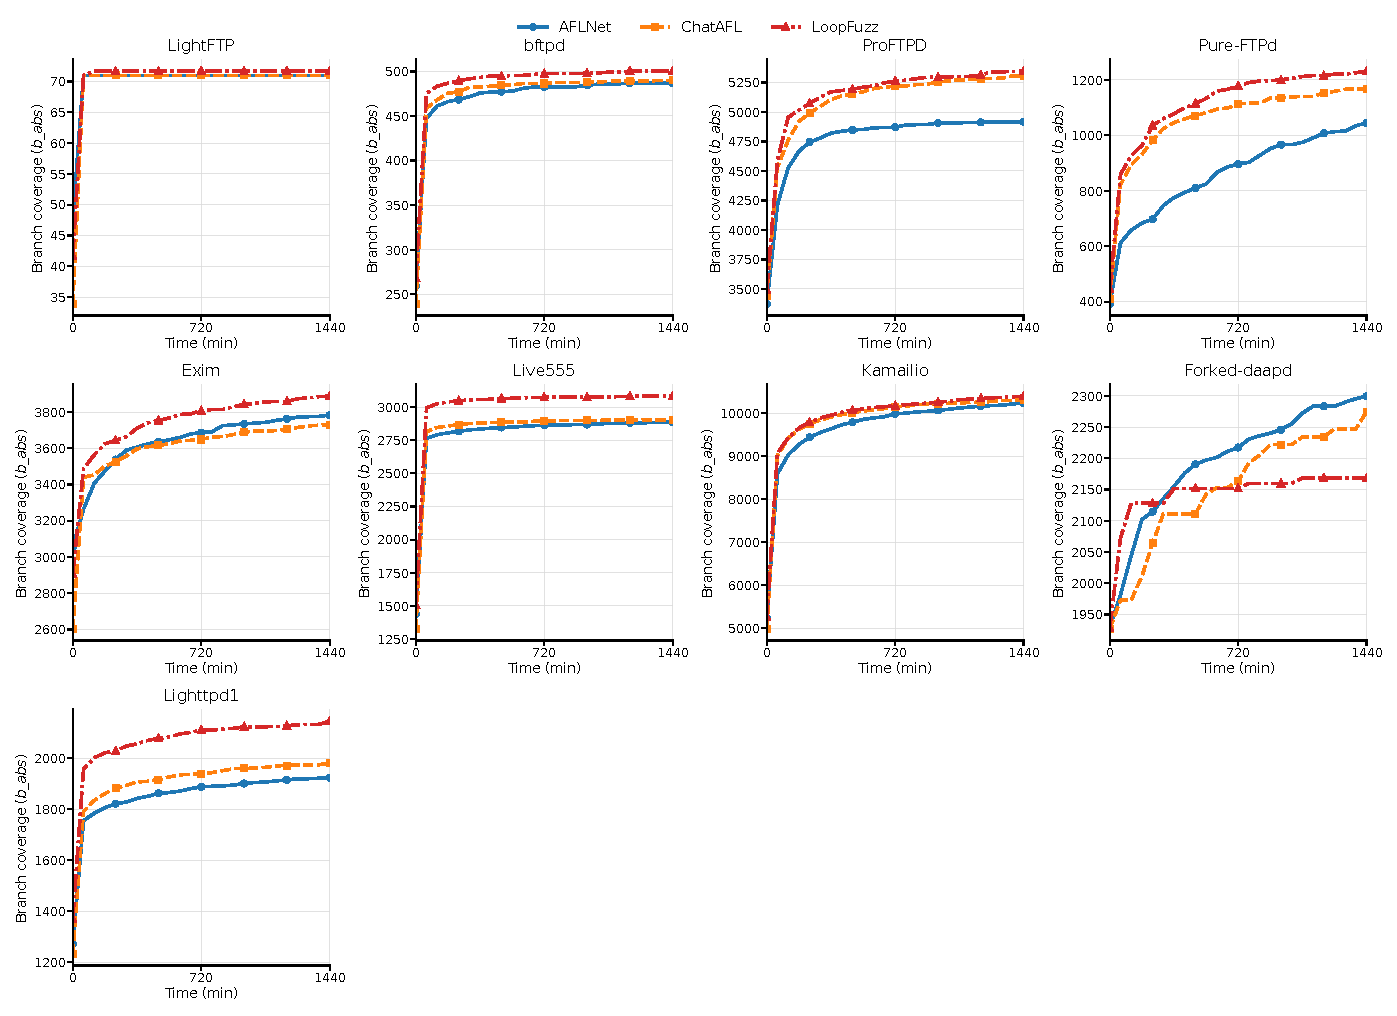
\includegraphics[width=\textwidth]{primary_branch_coverage_curve.pdf}
\caption{Branch-coverage trajectories for the nine primary-result targets. Each panel uses the same selected runs as Table~\ref{tab:24h_results}.}
\label{fig:primary_branch_curve}
\end{figure*}

\begin{figure*}[htbp]
\centering

\includegraphics[width=\textwidth]{primary_edge_exploration_curve.pdf}
\caption{IPSM-edge exploration trajectories for the nine primary-result targets. Each panel uses the same selected runs as Table~\ref{tab:24h_results}.}
\label{fig:primary_edge_curve}
\end{figure*}

\begin{table*}[!t]
\centering
\caption{Auxiliary NSFuzz branch-count artifacts. This table deliberately omits AFLNet, ChatAFL, and LoopFuzz columns; their same-build \texttt{b\_abs} values appear in Table~\ref{tab:24h_results}. The current package does not preserve enough NSFuzz-side build, instrumentation, and coverage-script metadata to certify metric identity on every target, so these NSFuzz counts are retained as external artifact diagnostics rather than as horizontal branch-coverage winners.}
\label{tab:aux_branch_results}
{\scriptsize
\setlength{\tabcolsep}{6.0pt}
\renewcommand{\arraystretch}{0.95}
\resizebox{0.46\textwidth}{!}{%
\begin{tabular}{l c}
\toprule
Target & NSFuzz artifact branch count \\
\midrule
LightFTP & $414.3 {\pm} 9.8$ \\
bftpd & $477.6 {\pm} 3.9$ \\
ProFTPD & $5335.0 {\pm} 86.9$ \\
Pure-FTPd & $1332.2 {\pm} 8.8$ \\
Exim & $4191.5 {\pm} 62.0$ \\
Live555 & $3021.5 {\pm} 42.1$ \\
Kamailio & $10635.3 {\pm} 123.8$ \\
Forked-daapd & $2722.8 {\pm} 44.6$ \\
\bottomrule
\end{tabular}}
}
\end{table*}

\begin{table*}[!t]
\centering
\caption{State-exploration diagnostics in the auxiliary archive. AFLNet, ChatAFL, and LoopFuzz report final response-derived AFLNet-lineage \texttt{edges}. The NSFuzz column reports \emph{NSFuzz artifact edge count} and is not horizontally comparable to those IPSM edge counts. Bold marks the highest mean only among AFLNet-lineage columns.}
\label{tab:aux_edge_artifact}
{\scriptsize
\setlength{\tabcolsep}{5.0pt}
\renewcommand{\arraystretch}{0.95}
\resizebox{0.86\textwidth}{!}{%
\begin{tabular}{l cccc}
\toprule
Target & AFLNet \texttt{edges} & ChatAFL \texttt{edges} & LoopFuzz \texttt{edges} & NSFuzz artifact edge count \\
\midrule
LightFTP & $182.8 {\pm} 10.2$ & $194.2 {\pm} 10.2$ & $\mathbf{216.6 {\pm} 10.4}$ & $11.0 {\pm} 0.0$ \\
bftpd & $166.9 {\pm} 9.4$ & $205.2 {\pm} 9.7$ & $\mathbf{221.7 {\pm} 16.9}$ & $48.7 {\pm} 4.8$ \\
ProFTPD & $180.5 {\pm} 23.1$ & $250.5 {\pm} 9.1$ & $\mathbf{271.7 {\pm} 18.8}$ & $186.0 {\pm} 11.5$ \\
Pure-FTPd & $213.9 {\pm} 11.9$ & $266.2 {\pm} 14.3$ & $\mathbf{291.0 {\pm} 23.6}$ & $17.6 {\pm} 0.5$ \\
Exim & $88.3 {\pm} 5.3$ & $116.4 {\pm} 10.2$ & $\mathbf{128.5 {\pm} 7.8}$ & $13.9 {\pm} 1.2$ \\
Live555 & $103.9 {\pm} 10.1$ & $151.2 {\pm} 3.9$ & $\mathbf{158.7 {\pm} 8.5}$ & $49.8 {\pm} 2.0$ \\
Kamailio & $101.1 {\pm} 7.7$ & $115.7 {\pm} 13.9$ & $\mathbf{127.6 {\pm} 9.6}$ & $14.3 {\pm} 0.7$ \\
Forked-daapd & $21.1 {\pm} 1.3$ & $20.5 {\pm} 2.1$ & $\mathbf{22.1 {\pm} 1.5}$ & $27.0 {\pm} 6.1$ \\
\bottomrule
\end{tabular}}
}
\end{table*}

\begin{table*}[!t]
\centering
\caption{MQTT/Mosquitto artifact-integrity summary. This table is not a performance ranking: the AFLNet row is a 24-hour AFLNet-lineage run, the LoopFuzz Mosquitto rows are much shorter, and MBFuzzer exposes \texttt{gcovr} branch coverage from a Mosquitto-only worker archive with no AFLNet-lineage \texttt{edges}.}
\label{tab:mqtt_artifact_integrity}
{\scriptsize
\setlength{\tabcolsep}{4.0pt}
\renewcommand{\arraystretch}{1.0}
\begin{tabularx}{\textwidth}{l c c c c X}
\toprule
Artifact & Runs & Runtime (min) & Branch metric & Edge metric & Use in this paper \\
\midrule
AFLNet Mosquitto & 10 & $1479.0 {\pm} 0.0$ & \texttt{b\_abs} $1814.3 {\pm} 147.3$ & \texttt{edges} $36.0 {\pm} 4.5$ & Same lineage but no ChatAFL row; excluded from the primary three-way table. \\
LoopFuzz Mosquitto & 10 & $137.4 {\pm} 134.7$ & \texttt{b\_abs} $2518.5 {\pm} 269.9$ & \texttt{edges} $107.7 {\pm} 18.1$ & Not same-budget with AFLNet; excluded from performance conclusions. \\
MBFuzzer Mosquitto & 10 & $\approx 1480$ & \texttt{gcovr} branches $2827.0 {\pm} 58.9$ & N/A & External Mosquitto-only artifact; no primary-format \texttt{b\_abs} or AFLNet-lineage \texttt{edges}. \\
\bottomrule
\end{tabularx}
}
\end{table*}

\subsection{RQ1: Whole-Campaign Effect}
LoopFuzz is evaluated here as an integrated control policy within the AFLNet and ChatAFL lineage, not as an isolated rejection heuristic or a replacement for all state-aware fuzzers. Table~\ref{tab:24h_results} and Fig.~\ref{fig:primary_branch_curve} show that direct open-loop assistance is not uniformly robust under the selected archived runs. ChatAFL ties AFLNet on LightFTP, finishes below AFLNet on Exim in \texttt{b\_abs}, is close to AFLNet on Forked-daapd, and improves several other targets. Under these conditions, improved generation alone does not consistently translate into stronger end-of-campaign coverage.

Within the primary AFLNet/ChatAFL lineage, LoopFuzz reaches the highest mean final \texttt{b\_abs} on eight of nine targets; AFLNet remains highest on Forked-daapd, where LoopFuzz also has much larger variance. After BH correction, LoopFuzz is higher than AFLNet on \texttt{b\_abs} for eight targets and lower on Forked-daapd, while its advantage over ChatAFL remains corrected-significant on five targets. The remaining positive mean separations over ChatAFL, such as bftpd, ProFTPD, and Kamailio, should be read as descriptive rather than inferential. Section~\ref{sec:forked_failure} analyzes Forked-daapd directly.

Table~\ref{tab:aux_branch_results} shows why NSFuzz artifacts are useful but not a homogeneous branch-coverage ranking. LightFTP reports $414.3{\pm}9.8$ NSFuzz artifact branches, while same-build AFLNet-lineage rows cluster around $71$. Forked-daapd is also diagnostic: NSFuzz reports $2722.8{\pm}44.6$, while AFLNet, ChatAFL, and LoopFuzz report $2326.3{\pm}77.3$, $2315.3{\pm}50.1$, and $2171.9{\pm}226.0$. The package lacks enough NSFuzz-side build and coverage-script metadata to certify metric identity, so these rows bound the claim rather than declare a cross-tool winner.

The LightFTP anomaly is especially instructive. The AFLNet-lineage LightFTP runs share the same target commit, \texttt{gcovr} replay script, \texttt{fftp} binary, and \texttt{ftpclean} reset path, yet branch coverage saturates near 71 within the first hour. The NSFuzz artifact is almost six times larger. Without NSFuzz-side build and replay metadata, the archive cannot distinguish stronger exploration from a different coverage surface. Section~\ref{sec:lightftp_anomaly} records the audit evidence and keeps this row out of the primary performance conclusion.

\subsection{RQ2: IPSM Escape Dynamics}

Terminal \texttt{edges} provide the clearest primary-lineage evidence for improved state exploration. In the AFLNet/ChatAFL comparison, LoopFuzz attains the highest mean on all nine primary targets, as visualized in Fig.~\ref{fig:primary_edge_curve}. After BH correction, the LoopFuzz-versus-AFLNet edge advantage remains significant on eight targets; Forked-daapd remains positive by mean but not significant. Against ChatAFL, the corrected edge advantage remains significant on six targets, while Kamailio, Forked-daapd, and Lighttpd1 are positive by mean but not corrected-significant.

Table~\ref{tab:aux_edge_artifact} keeps the NSFuzz edge archive separate from this state-exploration claim. AFLNet, ChatAFL, and LoopFuzz report response-derived IPSM edges, whereas the NSFuzz column is an artifact edge count from a different state-aware implementation. We therefore do not select an NSFuzz-versus-LoopFuzz edge winner from that table. The diagnostic mismatch is visible in the data: on LightFTP, NSFuzz has a much larger branch-count artifact in Table~\ref{tab:aux_branch_results} but an artifact edge count of only $11.0{\pm}0.0$; on Forked-daapd, NSFuzz reports $27.0{\pm}6.1$ artifact edges while the AFLNet-lineage edge counts are $21.1{\pm}1.3$, $20.5{\pm}2.1$, and $22.1{\pm}1.5$. These values may be useful for reproducing the archive, but they are not a common semantic edge metric.

\subsection{RQ3: End-of-Campaign Outcome}

The \texttt{b\_abs} comparison is less uniform even before considering external artifacts. In the primary three-way comparison, LoopFuzz is strongest by mean on most targets but does not lead Forked-daapd. The NSFuzz branch-count artifacts add boundary evidence rather than a homogeneous ranking: the LightFTP and Forked-daapd artifact counts are much larger than the AFLNet-lineage branch counts, but the archive does not prove that the same build, instrumentation, replay harness, and coverage extraction surface were used. Table~\ref{tab:mqtt_artifact_integrity} shows a different boundary for Mosquitto: MBFuzzer has a recoverable \texttt{gcovr} branch count, but no AFLNet-lineage \texttt{b\_abs}/\texttt{edges}, and the LoopFuzz Mosquitto rows are much shorter than 24 hours. The \texttt{edges} result has a narrower scope: it supports improved response-derived IPSM exploration within the AFLNet/ChatAFL lineage, but the NSFuzz artifact edge counts and MBFuzzer Mosquitto artifacts cannot extend or negate that claim because they are not the same measurement. This distinction matters for interpretation: the audited archive supports improved state exploration within the closest lineage and a selective absolute-branch-coverage advantage on the primary targets, not a blanket dominance claim over specialized fuzzers.

\subsection{Artifact Anomaly: LightFTP}
\label{sec:lightftp_anomaly}

LightFTP is the largest metric-consistency warning in the auxiliary archive. In the primary table, all three AFLNet-lineage systems use the same LightFTP build and coverage-replay path. The local Dockerfile checks out LightFTP commit \texttt{139af7c}; the fuzzing build uses \texttt{AFL\_USE\_ASAN=1 CC=afl-clang-fast}; the coverage build applies the local \texttt{gcov.patch} and compiles with \texttt{-fprofile-arcs -ftest-coverage}; and the coverage script replays queue entries against \texttt{fftp}, runs \texttt{gcovr -r ..}, and resets the shared FTP directory through \texttt{ftpclean}. Under that path, the branch-coverage trajectory reaches $71.0$ by 60 minutes for AFLNet and ChatAFL, and $71.7$ by 120 minutes for LoopFuzz, then remains flat through 1440 minutes.

The NSFuzz artifact for the same nominal target is $414.3{\pm}9.8$ branch-count units. The current archive does not include the NSFuzz-side LightFTP Dockerfile, target commit confirmation, patch set, compiler and coverage flags, replay harness, or coverage extraction script. Because those fields are missing, we cannot tell whether the NSFuzz artifact reflects a stronger exploration strategy on the identical LightFTP coverage surface or a different target build, instrumentation scope, input model, or counting script. The accompanying NSFuzz artifact edge count is also only $11.0{\pm}0.0$, which reinforces that the NSFuzz state/edge artifact is not the AFLNet-lineage response-derived IPSM metric.

We therefore make a conservative choice. LightFTP remains in Table~\ref{tab:24h_results} for the AFLNet/ChatAFL/LoopFuzz lineage comparison, where the build and coverage pipeline are shared. The NSFuzz LightFTP value remains in Table~\ref{tab:aux_branch_results} as an external artifact anomaly that future work should re-run under a common Dockerfile and coverage script. It is not used as evidence that NSFuzz opened extra branches in the identical LightFTP build, nor as evidence that LoopFuzz is inferior to NSFuzz on a certified common branch-coverage metric.

\subsection{Failure-Target Analysis: Forked-daapd}
\label{sec:forked_failure}

Forked-daapd is the clearest primary failure target for LoopFuzz. In Table~\ref{tab:24h_results}, LoopFuzz ends at $2171.9{\pm}226.0$ final \texttt{b\_abs}, below AFLNet at $2326.3{\pm}77.3$ and ChatAFL at $2315.3{\pm}50.1$. The variance is also diagnostic: LoopFuzz's branch-coverage standard deviation is about three times AFLNet's and more than four times ChatAFL's. Table~\ref{tab:aux_branch_results} also reports a high NSFuzz artifact branch count of $2722.8{\pm}44.6$ for this target, but we do not treat that value as a certified same-pipeline comparison. The same target therefore bounds both claims: LoopFuzz can improve response-derived IPSM exploration while still missing branch coverage reached by the simpler AFLNet-lineage baseline, and the external artifact suggests that stronger state-aware strategies may expose additional behavior under conditions that require re-audit.

The trajectory evidence points to a state-signal mismatch rather than a slow start. LoopFuzz is ahead after 60 minutes on Forked-daapd ($2072.5$ \texttt{b\_abs}) while AFLNet and ChatAFL are at $1981.6$ and $1973.1$. It then plateaus at $2168.6$ from 1080 to 1440 minutes, while AFLNet rises from $2272.3$ to $2299.5$ and ChatAFL from $2234.3$ to $2274.7$. The edge trajectory has the opposite shape: LoopFuzz reaches $17.9$ IPSM edges by 60 minutes, versus $11.9$ and $11.7$, and ends slightly higher at $22.1$. Thus, faster response-derived state growth does not translate into deeper branch exploration on this target.

A plausible explanation is that DAAP/DACP exposes a noisy or sparse response signal for the AFLNet-lineage IPSM abstraction. Forked-daapd contains media-library and control-session behavior where requests can change visible responses without exercising branches that dominate \texttt{b\_abs}. LoopFuzz may therefore promote candidates that look state-progressive but are not branch-productive. The high variance is also compatible with initialization or early-history instability, although the archive lacks per-run server-state logs to confirm that mechanism.

The ablation row does not support a simple ``one switch is too strict'' explanation. On Forked-daapd, removing CEGR, frontier scheduling, hypothesis validation, or adaptive triggering all lowers \texttt{b\_abs} relative to the full controller (-104.4, -145.0, -129.9, and -91.8). Some relaxed variants slightly increase \texttt{edges}, but not branch coverage. This means the failure is unlikely to be fixed merely by disabling one exposed sub-control. More likely, the target needs a different admission signal, such as richer DAAP/DACP response parsing, target-state normalization, database/session initialization checks, or a \emph{LoopFuzz-no-admission} run to test whether model suggestions are being rejected too aggressively or are simply unhelpful for this protocol.

\subsection{Ablation: Boundary-Condition Analysis}

Table~\ref{tab:ablation_results} reports the archived policy perturbations as deltas relative to the evaluated full controller. Each cell shows $\Delta$ \texttt{b\_abs} / $\Delta$ \texttt{edges}. These rows should not be read as a no-admission experiment: none preserves the same model-call path while bypassing the full $P/U/R/G$ admission formula and directly accepting model suggestions. The updated archive therefore supports only an integrated-policy interpretation.

Within that scope, the ablation table is best read as a boundary-condition analysis rather than as a monotone proof that every switch is always beneficial. The clearest stable signal is frontier control: removing it reduces mean \texttt{b\_abs} on all nine targets, which suggests that state-directed budget allocation is broadly useful in this archive. The remaining switches are more target-dependent.

CEGR is the main non-monotone case. Removing CEGR increases \texttt{b\_abs} on ProFTPD by +99.1 and on Live555 by +1.2, while reducing \texttt{edges} on both targets (-5.2 and -1.5). This pattern is consistent with CEGR sometimes over-constraining the local message space: a repaired hypothesis can prevent repeated invalid continuations, but it can also narrow a target-specific region where looser mutations still reach additional instrumented branches. On the other seven targets, removing CEGR reduces \texttt{b\_abs}, so the archive does not show that CEGR is generally harmful. It shows a boundary condition: local repair helps most primary targets, but ProFTPD and Live555 may need a less aggressive repair policy or a decay mechanism that reopens constraints after they stop producing coverage.

Adaptive triggering shows a different boundary condition. Removing it improves both \texttt{b\_abs} and \texttt{edges} on Pure-FTPd (+6.3/+10.7) and Kamailio (+26.9/+5.2), and improves \texttt{b\_abs} but not \texttt{edges} on Live555 (+5.0/-3.6). For LightFTP, ProFTPD, and Lighttpd1, the same switch raises \texttt{edges} but lowers \texttt{b\_abs}. These mixed deltas suggest that the plateau trigger can be too late or too conservative for targets where earlier model intervention exposes useful request variants, but that more intervention can also expand response-derived state structure without translating into branch coverage. Because the current archive lacks per-target model-call and admission-event counts, we treat this as a diagnostic interpretation rather than as a quantified mechanism claim.

Disabling hypothesis validation has the same cautionary shape: \texttt{b\_abs} drops on every target, yet \texttt{edges} rises on Pure-FTPd, Kamailio, and Forked-daapd. This reinforces that a larger response-derived IPSM is not automatically a better campaign endpoint. The complete strategy is therefore reasonably robust as an integrated policy, especially for branch coverage under frontier control, but individual components remain target-dependent. A future \emph{LoopFuzz-no-admission} run would still be required to isolate whether the full admission boundary, holding model calls and scheduling fixed, is the dominant causal factor.

\begin{table*}[!t]
\centering
\caption{Policy-perturbation results relative to the evaluated full controller. The table does not include a \emph{LoopFuzz-no-admission} condition that preserves model calls and scheduling while bypassing the full $P/U/R/G$ admission checks. The first number in each cell is final \texttt{b\_abs}; the second is final \texttt{edges}. The Full column reports mean final \texttt{b\_abs} / \texttt{edges}; other cells report deltas relative to that mean. Runs with archived runtime below 1400 minutes are excluded; when more than 10 valid runs remain, we keep the lowest 10 run IDs. Some ablated target-policy cells contain seven to nine eligible runs after this filter.}
\label{tab:ablation_results}
{\scriptsize
\setlength{\tabcolsep}{2.8pt}
\renewcommand{\arraystretch}{0.95}
\resizebox{\textwidth}{!}{%
\begin{tabular}{l c c c c c}
\toprule
Target & Full & No CEGR & No frontier & No hypothesis & No adaptive trigger \\
\midrule
LightFTP & 71.6 / 213.9 & -0.2 / -13.5 & -0.6 / -14.5 & -0.5 / -11.0 & -0.6 / +1.8 \\
bftpd & 501.5 / 221.7 & -3.1 / -7.5 & -3.0 / -8.4 & -5.2 / -5.0 & -7.0 / -12.1 \\
ProFTPD & 5358.8 / 271.7 & +99.1 / -5.2 & -118.7 / -37.3 & -8.3 / +0.1 & -20.6 / +0.4 \\
Pure-FTPd & 1242.6 / 291.0 & -19.2 / +1.1 & -18.9 / -1.4 & -0.6 / +15.9 & +6.3 / +10.7 \\
Exim & 3908.5 / 128.5 & -29.0 / -2.8 & -40.7 / -2.8 & -43.0 / -3.3 & -40.6 / -8.9 \\
Live555 & 3088.7 / 158.7 & +1.2 / -1.5 & -21.0 / -9.6 & -12.2 / -4.4 & +5.0 / -3.6 \\
Kamailio & 10402.7 / 127.6 & -96.7 / +2.5 & -121.4 / -5.0 & -100.6 / +1.9 & +26.9 / +5.2 \\
Forked-daapd & 2171.9 / 22.1 & -104.4 / -0.9 & -145.0 / +0.1 & -129.9 / +0.7 & -91.8 / -1.7 \\
Lighttpd1 & 2156.5 / 32.5 & -62.4 / -3.3 & -15.9 / +1.9 & -33.9 / -2.4 & -27.1 / +4.1 \\
\bottomrule
\end{tabular}}
}
\end{table*}

\section{Discussion}

The paper makes one central design claim. In stateful protocol fuzzing, LLM generation should be governed by runtime evidence before it changes a campaign. ChatAFL already showed that an LLM can generate protocol text~\cite{chatafl}. LoopFuzz asks a different question: when should such output be trusted by the campaign? Our design answer is closed-loop runtime admission control. It checks structure and parseability before a trial, then uses the trial response, state movement, and coverage gain to decide whether an LLM suggestion can strengthen the queue. The present archive supports this design as part of an integrated control strategy, but it does not contain the no-admission ablation needed to prove the admission boundary's independent effect.

The admission controller and the scheduler solve different parts of the same problem. Admission control filters low-value suggestions. It does not decide where to spend the recovered budget. State-aware scheduling decides where to search. Without closed-loop intervention, however, it still depends on ordinary mutation to cross semantic bottlenecks. LoopFuzz combines the two because admission control and state-directed search reinforce each other.

The results also show why response-derived state counts must be read carefully. A campaign can accumulate superficially different rejection paths without moving toward high-value logic. LoopFuzz therefore reads state exploration together with \texttt{b\_abs} and demotes states that remain unproductive over repeated selections. In this setting, productive states matter more than raw state counts. For that reason, \texttt{edges} is best interpreted as a companion diagnostic for campaign behavior, not as a substitute for absolute branch coverage.

Forked-daapd is the strongest example of this limitation. LoopFuzz grows the response-derived IPSM faster and ends with slightly more primary-lineage \texttt{edges}, but it underperforms AFLNet and ChatAFL in final branch coverage; the NSFuzz artifact branch count is also much higher and should be re-audited under a common pipeline. This outcome suggests that DAAP/DACP response-level progress can be too weak or noisy for the current admission and scheduling policy. It also shows why the paper's claim must remain scoped to the evaluated lineage and outcome mix rather than being framed as universal improvement.

The present method is evaluated on textual or semi-textual protocols whose message regions can be parsed cheaply and whose responses provide useful progress signals. That scope covers the benchmark suite used here and many request-response protocols of practical interest. Opaque binary or encrypted protocols require stronger parsers, auxiliary instrumentation, or richer response abstractions. Response codes alone may not expose state reachability in those settings. That extension matters, but it lies beyond the current empirical scope.

The present evaluation is also centered on campaign-control behavior rather than on vulnerability yield. We preserve crashes and queue artifacts, but we do not report new CVEs or newly confirmed bugs in this study because crash deduplication, exploitability review, and cross-target triage remain incomplete under one uniform protocol. The paper should therefore be read as evidence about campaign control and exploration quality, not as an end-to-end demonstration of stronger bug-finding yield.

Counterexample-guided local refinement is also a deliberate design choice. Repeated unconstrained regeneration does not accumulate persistent knowledge. Local refinement turns failed executions into stored evidence. It makes runtime evidence cumulative rather than disposable. The boundary-condition analysis, however, shows that this repair pressure can be target-dependent. On ProFTPD and Live555, disabling CEGR raises \texttt{b\_abs} while lowering \texttt{edges}, which suggests that local repairs may sometimes over-shrink a search region that still contains branch-productive variants. Adaptive triggering has a related boundary condition: on Pure-FTPd and Kamailio, earlier or less conservative intervention appears to help both reported endpoints, whereas on other targets it mainly changes response-derived state structure. These observations do not invalidate the integrated controller, but they do prevent a stronger claim that each component is independently necessary on every protocol. The complete strategy is best characterized as broadly robust with target-dependent sub-controls.

\section{Threats to Validity}
\label{sec:threats}

\textbf{Internal validity:} LLM-assisted fuzzing remains sensitive to generation variance, target nondeterminism, and timing effects. We mitigate these threats by fixing the environment, pinning the model endpoint, using low temperatures for grammar extraction and refinement, and using repeated 24-hour runs. Each archived run is isolated in a Docker container with a one-CPU quota and separate network namespace. However, the artifact lacks the global co-scheduling plan, host-load trace, Docker \texttt{stats}, CPU-frequency trace, and per-run PRNG seeds. It therefore cannot rule out residual wall-clock effects from contention, storage pressure, network jitter, or scheduler decisions. Growth-rate plots are descriptive wall-clock traces, not CPU-time-normalized throughput claims. Plateau triggering and refinement are history-dependent, so the study cannot cleanly separate model variance from control-policy variance.

\textbf{Statistical conclusion validity:} The primary table spans nine targets, two endpoint metrics, and two LoopFuzz-versus-baseline comparisons per metric. Table~\ref{tab:primary_stats} reports raw Mann-Whitney $p$ values, BH-adjusted $q$ values, and Cliff's $\delta$ for all 36 tests from the selected per-run endpoint vectors. These tests are still limited by small sample size ($n=10$ per cell), ties in some endpoint distributions, and the fact that the deterministic run-selection rule is based on recoverable archive rows rather than a complete launch ledger. We therefore interpret corrected-significant rows as endpoint evidence within the audited archive, not as universal target behavior.

\textbf{External validity:} The benchmark suite spans 10 implementations across seven protocol families, but the primary three-way comparison covers the nine non-MQTT targets with comparable AFLNet, ChatAFL, and LoopFuzz rows. Evidence is strongest for textual or semi-textual protocols whose progress is visible in responses and for systems sharing the AFLNet/ChatAFL response-derived IPSM lineage. We do not claim unchanged transfer to opaque binary or encrypted protocols, nor superiority over all state-aware fuzzers. The archive lacks same-format StateAFL, Bleem, and Logos reproductions under the same selection rule. NSFuzz artifact rows are target-specific diagnostics rather than a unified cross-system state-machine comparison, and MBFuzzer is available only as a Mosquitto worker archive without AFLNet-lineage \texttt{edges}.

\textbf{Construct validity:} We use final \texttt{b\_abs} and final \texttt{edges} as proxies for fuzzing effectiveness, but neither fully captures semantic protocol progress. AFLNet-lineage \texttt{b\_abs} rows use shared target and replay pipelines, while NSFuzz branch counts remain artifact counts unless their build, instrumentation, and coverage extraction can be audited; the LightFTP $414.3{\pm}9.8$ artifact shows why this distinction matters. Runtime admission means structured output checks, bounded validation executions, response-grounded acceptability, state-reachability signals, and CEGR, not formal verification or a perfect pre-execution oracle. The ablation archive also lacks \emph{LoopFuzz-no-admission}, and event-level admission logs are unavailable. Semantic drift is therefore specified operationally and illustrated by a trace, not quantified as a cross-target prevalence or acceptance rate.

\textbf{Reproducibility validity:} ChatAFL and LoopFuzz share the same pinned model endpoint, each primary target is drawn from one declared archive, and the paper states the deterministic run-selection rule. Scripts document container isolation, CPU and memory quotas, internal ports, timeout handling, result manifests, and recovery logic. Table~\ref{tab:run_filtering_inventory} reports the recoverable selected inventory, but the artifact lacks full pre-filter inventories and failure metadata for any runs not represented in the selected cache. Mosquitto/MQTT rows are excluded from performance conclusions because they lack a homogeneous comparison surface: LoopFuzz averages 137.4 minutes, AFLNet and MBFuzzer are close to 1480 minutes, and MBFuzzer exposes worker-level \texttt{gcovr} branch coverage rather than AFLNet-lineage \texttt{b\_abs}/\texttt{edges}. A complete package should also preserve fuzzer statistics, stall-interaction logs, raw prompts and replies, admission decisions, rejection reasons, refinement events, latency, token counters, exclusion logs, launch manifests, batch schedules, resource traces, and PRNG seeds.

\section{Conclusion}
This evaluation supports a bounded design lesson: fluent protocol text is insufficient for a stateful campaign. In the evaluated AFLNet and ChatAFL lineage, the integrated LoopFuzz control strategy combines runtime admission, local refinement, and state-aware scheduling to reduce the risk of semantically premature model suggestions.

Under the audited primary AFLNet and ChatAFL lineage comparison, LoopFuzz's clearest effect is improved state exploration, with a selective branch-coverage advantage on the same benchmark archive. Mean final response-derived IPSM \texttt{edges} improves across the nine off-the-shelf primary targets; after correction, the advantage remains significant on eight targets versus AFLNet and six targets versus ChatAFL. Mean final \texttt{b\_abs} improves on eight of nine primary targets versus AFLNet and on eight of nine versus ChatAFL by mean, with corrected significance on eight and five targets respectively. Forked-daapd remains the primary-target exception for branch coverage.

The broader baseline picture is mixed and incomplete. NSFuzz artifact counts are informative external diagnostics, especially on LightFTP and Forked-daapd, but the current package does not preserve enough NSFuzz-side build, instrumentation, replay, and coverage-extraction metadata to treat those rows as homogeneous \texttt{b\_abs} rankings. MBFuzzer is recoverable only as a Mosquitto worker artifact with \texttt{gcovr} branch coverage and no AFLNet-lineage \texttt{edges}. Forked-daapd is the clearest primary negative target: LoopFuzz shows faster early response-derived state growth there, but its branch coverage plateaus below AFLNet and ChatAFL; the higher NSFuzz artifact count should be re-audited under a common pipeline. Same-format StateAFL, Bleem, and Logos reproductions are not available in the current archive. The archived ablations show a robust integrated strategy but target-dependent sub-controls: CEGR can over-constrain ProFTPD and Live555 branch exploration, and adaptive triggering can be too conservative on Pure-FTPd and Kamailio. They also lack the \emph{LoopFuzz-no-admission} condition needed to isolate the full admission boundary. The evidence therefore supports a precise conclusion: the integrated LoopFuzz control strategy improves state-exploration behavior within the closest AFLNet/ChatAFL lineage and improves absolute branch coverage on most primary targets, but this study does not establish the independent causal effect of the complete admission formula, per-module necessity on every target, or dominance over specialized external fuzzers.

\section*{CRediT authorship contribution statement}
Author contribution roles must be confirmed by all authors before submission. A conservative draft is maintained in \texttt{AUTHOR\_DECLARATIONS\_TO\_CONFIRM.md} for transfer into Editorial Manager or into this section after confirmation.

\section*{Declaration of competing interest}
The competing-interest declaration must be confirmed by all authors before submission. A draft declaration is maintained in \texttt{AUTHOR\_DECLARATIONS\_TO\_CONFIRM.md}.

\section*{Funding}
Funding information must be confirmed by all authors before submission. A draft funding statement is maintained in \texttt{AUTHOR\_DECLARATIONS\_TO\_CONFIRM.md}.

\section*{Data availability}
Data and code availability statements must be confirmed before submission. The current artifact contains local run summaries and analysis scripts, but no public repository URL or DOI is declared in this manuscript.

\section*{Declaration of Generative AI and AI-assisted technologies in the manuscript preparation process}
During the preparation of this work, the authors used OpenAI Codex for language editing, LaTeX formatting, and submission-compliance checking. After using this tool, the authors reviewed and edited the content as needed and take full responsibility for the content of the publication.

\setlength{\bibsep}{0pt}
\bibliographystyle{elsarticle-num-names}
\bibliography{references}

\end{document}
